\documentclass[11pt]{article} % Anonymized submission
% \renewcommand{\includegraphics}[1][1]{}

\usepackage[nonatbib]{neurips_2021}

% The following packages will be automatically loaded:
% amsmath, amssymb, natbib, graphicx, url, algorithm2e

\usepackage{times}
\usepackage{lmodern}
\usepackage{hyperref}       % hyperlinks  %[implicit=false, bookmarks=false]
\usepackage{booktabs}       % professional-quality tables
\usepackage{amsfonts,amsmath,amssymb,amsthm}       % blackboard math symbols
\usepackage{nicefrac}       % compact symbols for 1/2, etc.
\usepackage{microtype}      % microtypography
\usepackage{graphicx}
\usepackage{sidecap}

\usepackage[numbers, sort, compress]{natbib}

\usepackage{mathtools, verbatim}
%\usepackage[thmmarks, thref, amsthm]{ntheorem}
%\usepackage{color}
\usepackage[dvipsnames]{xcolor}
\definecolor{darkblue}{rgb}{0.0,0.0,0.2}
\hypersetup{colorlinks,breaklinks,
	linkcolor=darkblue,urlcolor=darkblue,
	anchorcolor=darkblue,citecolor=darkblue}
\definecolor{myblue}{rgb}{0,0.3,0.8} \definecolor{myorange}{rgb}{0.9,0.5,0}
\usepackage{wrapfig}
\usepackage[small]{caption}
\usepackage[colorinlistoftodos,textsize=tiny]{todonotes} % need xargs for below
%\usepackage{accents}
\usepackage{bbm}
\usepackage{xspace}

\usepackage{tikz,pgfplots,tikz-3dplot}
\usetikzlibrary{arrows.meta,shapes.misc,positioning,fit,calc,intersections,through,decorations.markings}
\tdplotsetmaincoords{55}{135}        % for simplex diagrams

\tikzstyle{cell}=[dashed,thick]
\tikzstyle{simplex}=[thick]
\newcommand{\tikzfigscale}{2.2}
\newcommand{\placefiglabel}[1]{\node at (1.1,0,1.7) {#1};}
\usetikzlibrary{arrows}
\usetikzlibrary{shapes}


\makeatletter
\let\Ginclude@graphics\@org@Ginclude@graphics 
\makeatother

%\usetikzlibrary{calc}
\newcommand{\Comments}{1}
\newcommand{\mynote}[2]{\ifnum\Comments=1\textcolor{#1}{#2}\fi}
\newcommand{\mytodo}[2]{\ifnum\Comments=1%
	\todo[linecolor=#1!80!black,backgroundcolor=#1,bordercolor=#1!80!black]{#2}\fi}
\newcommand{\raf}[1]{\mynote{green}{[RF: #1]}}
\newcommand{\raft}[1]{\mytodo{green!20!white}{RF: #1}}
\newcommand{\jessie}[1]{\mynote{purple}{[JF: #1]}}
\newcommand{\jessiet}[1]{\mytodo{purple!20!white}{JF: #1}}
\newcommand{\bo}[1]{\mynote{blue}{[Bo: #1]}}
\newcommand{\botodo}[1]{\mytodo{blue!20!white}{[Bo: #1]}}
\newcommand{\btw}[1]{}%\mytodo{orange!80!white}{BTW: #1}}
\newcommand{\discuss}[1]{\mynote{cyan!20!white}{#1}}
\ifnum\Comments=1               % fix margins for todonotes
\setlength{\marginparwidth}{1in}
\fi

\newcommand{\reals}{\mathbb{R}}
\newcommand{\posreals}{\reals_{>0}}%{\reals_{++}}
\newcommand{\simplex}{\Delta_\Y}
\newcommand{\relint}[1]{\mathrm{relint}(#1)}
\newcommand{\interior}{\mathrm{int}\,}
\newcommand{\prop}[2][\mathcal{P}]{\mathrm{prop}_{#1}[#2]}
\newcommand{\elic}{\mathrm{elic}}
\newcommand{\eliccvx}{\mathrm{elic}_\mathrm{cvx}}
\newcommand{\conscvx}{\mathrm{cons}_\mathrm{cvx}}
\newcommand{\elicpoly}{\mathrm{elic}_\mathrm{pcvx}}
\newcommand{\elicembed}{\mathrm{elic}_\mathrm{embed}}
\newcommand{\ccdim}{\mathrm{cc\,dim}}
\newcommand{\rank}{\mathrm{rank}}
\newcommand{\proj}{\mathrm{proj}}
\newcommand{\supp}{\mathrm{supp}}
\newcommand{\spn}{\mathrm{span}}

\newcommand{\range}{\mathrm{range}\,}
\newcommand{\zeros}[1]{\mathrm{ker}_\P\,#1}
\newcommand{\codim}{\mathrm{codim}}
\newcommand{\Pcodim}{\mathcal{P}\!\text{-}\mathrm{codim}}
\newcommand{\Pcodimension}{$\mathcal{P}$-codimension\,}

\newcommand{\propdis}{\mu}
\newcommand{\affhull}{\mathrm{affhull}}
\newcommand{\epi}{\mathrm{epi}}
\newcommand{\cl}{\mathbf{cl}}
%\newcommand{\span}{\mathrm{span}}

\newcommand{\A}{\mathcal{A}}
\newcommand{\C}{\mathcal{C}}
\newcommand{\D}{\mathcal{D}}
\newcommand{\E}{\mathbb{E}}
\newcommand{\F}{\mathcal{F}}
\renewcommand{\L}{\mathcal{L}}
\newcommand{\Lcvx}{\mathcal{L}^{\mathrm{cvx}}}
\newcommand{\I}{\mathcal{I}}
\newcommand{\N}{\mathcal{N}}
\newcommand{\R}{\mathcal{R}}
\renewcommand{\P}{\mathcal{P}}
\newcommand{\Sc}{\mathcal{S}}  % jessie, feel free to redef, just not \S :-)
\newcommand{\Scr}{\mathcal{S}}  % using this for the span of F_p - not sure if we want this to be parallel to the feasible subspace notation
\newcommand{\U}{\mathcal{U}}
\newcommand{\V}{\mathcal{V}}
\newcommand{\X}{\mathcal{X}}
\newcommand{\Y}{\mathcal{Y}}


\newcommand{\ellbar}{\underline{\ell}}
\newcommand{\lbar}{\underline{L}} % couldn't do L* while proofreading...
\newcommand{\iden}{\mathrm{iden}}
\newcommand{\im}{\mathrm{im}}
\newcommand{\Var}{\mathrm{Var}}
\newcommand{\CVaR}{\mathrm{CVaR}}

\newcommand{\exploss}[3]{\E_{#3} #1(#2,Y)}
\newcommand{\risk}[1]{\underline{#1}}
\newcommand{\Ind}[1]{\mathbf{I}\{{#1}\}}
\newcommand{\inprod}[2]{\langle #1, #2 \rangle}
\newcommand{\toto}{\rightrightarrows}
\newcommand{\ones}{\mathbbm{1}}

\newtheorem{theorem}{Theorem}
\newtheorem{lemma}{Lemma}
\newtheorem{proposition}{Proposition}
\newtheorem{corollary}{Corollary}
\newtheorem{conjecture}{Conjecture}
\newtheorem{definition}{Definition}
\newtheorem{assumption}{Assumption}
\newtheorem{condition}{Condition}
\newtheorem{remark}{Remark}


\DeclareMathOperator*{\argmax}{arg\,max}
\DeclareMathOperator*{\argmin}{arg\,min}
\DeclareMathOperator*{\arginf}{arg\,inf}
\DeclareMathOperator*{\sgn}{sgn}

\usepackage{thmtools, thm-restate}
%\declaretheorem{corollary}



% The \author macro works with any number of authors. There are two commands
% used to separate the names and addresses of multiple authors: \And and \AND.
%
% Using \And between authors leaves it to LaTeX to determine where to break the
% lines. Using \AND forces a line break at that point. So, if LaTeX puts 3 of 4
% authors names on the first line, and the last on the second line, try using
% \AND instead of \And before the third author name.

%Indirect elicitation as a necessary condition for consistent surrogate losses
\title{Unifying Lower Bounds on Prediction Dimension of Consistent Convex Surrogates}

\author{%
	Jessie Finocchiaro\thanks{Use footnote for providing further information
		about author (webpage, alternative address)---\emph{not} for acknowledging
		funding agencies.} \\
	Department of Computer Science\\
	CU Boulder\\
	\texttt{jefi8453@colorado.edu} \\
	% examples of more authors
	\And
	Raf Frongillo \\
	CU Boulder \\
	\texttt{raf@colorado.edu} \\
	\AND
	Bo Waggoner\\
	CU Boulder \\
	\texttt{bwag@colorado.edu} \\
	% \And
	% Coauthor \\
	% Affiliation \\
	% Address \\
	% \texttt{email} \\
	% \And
	% Coauthor \\
	% Affiliation \\
	% Address \\
	% \texttt{email} \\
}



\begin{document}

\maketitle

\begin{abstract}
The prediction dimension of a supervised learning task is the lowest dimension $d$ such that there exists a convex surrogate $L : \mathbb{R}^d \times \mathcal{Y} \to \mathbb{R}$ that is consistent for the given task.
  We present a new tool based on property elicitation, $d$-flats, for lower-bounding prediction dimension.
  This tool unifies approaches from a variety of domains, including continuous and discrete prediction problems.
  We use $d$-flats to obtain a new lower bound on the prediction dimension of risk measures, addressing an open question due to Frongillo and Kash (NeurIPS 2015).
  In discrete prediction settings, we show that the $d$-flats approach recovers and even tightens previous lower bounds using feasible subspace dimension.
\end{abstract}

\section{Introduction}\label{sec:intro}
%supervised learning blah
A surrogate loss function is an error measure that is related but not identical to one's target problem of interest.
Selecting a hypothesis by minimizing surrogate risk is one of the most widespread techniques in supervised machine learning.
There are two main reasons why a surrogate loss is necessary: (I) the target loss does not satisfy some desiderata, such as convexity, or (II) the goal is to estimate some target statistic and there is no target loss, as in many continuous estimation problems.
%(1) often occurs in discrete settings such as classification, while (2) is commone in continuous prediction problems when one seeks to estimate a target conditional statistic.%\raft{I felt we needed a sentence like this to justify \emph{why} we need a surrogate. And given that we need it, we can't really avoid hinting at the quadrants...}
In both settings, a key criteria for choosing a surrogate loss is \emph{consistency}, a precursor to excess risk bounds and convergence rates.
Roughly speaking, consistency means that minimizing surrogate risk corresponds to solving the target problem of interest, i.e. in (I) the target risk is also minimized, or in (II) the continuous prediction approaches the true conditional statistic.

% examples of problems where we care a lot about prediction dimension (that happen to be finite discrete)
Despite the ubiquity of surrogate losses, we lack general frameworks to design and analyze consistent surrogates.
This state of affairs is especially dire when one seeks low \emph{prediction dimension}, the dimension of the surrogate prediction domain.
For example, in multiclass classification with $n$ labels, the prediction domain might be $\reals^n$.
In many type (I) settings, such as structured prediction and extreme classification, the prediction dimension can easily become intractably large, forcing one to sacrifice consistency for computational efficiency.
To understand whether this sacrifice is necessary, recent work developed tools like the feasible subspace dimension to lower bound the prediction dimension of any consistent convex surrogate~\citep{ramaswamy2016convex}.
Challenges of type (II) include estimating risk measures such as conditional value at risk (CVaR), with applications in financial regulation, robust engineering design, and algorithmic fairness.
Risk measures are not elicitable, meaning they cannot be specified via a \jessiet{discrete? this sentence confuses me as is because the surrogate could be the target?}\raft{better?} target loss, and thus we seek a surrogate loss of low (or at least finite) prediction dimension.
Recent work~\citep{fissler2016higher,frongillo2020elicitation} gives prediction dimension bounds for some of these risk measures, but without the requirement that the surrogate be convex; bounds for convex surrogates are left as a major open question.

We present a new tool, \emph{$d$-flats}, which unifies existing techniques to bound the prediction dimension of consistent convex surrogates in both settings above.
Using this tool, we give the first prediction dimension bounds for risk measures with respect to convex surrogates, addressing the open question for type (II) above.
In settings of type (I), $d$-flats recover and tighten the feasible subspace dimension result of \citet{ramaswamy2016convex}.
%In settings of type (I), $d$-flats give tighter bounds in some cases, e.g. feasible subspace dimension result of \citet{ramaswamy2016convex}.
% Applied to settings of type (1), we recover the feasible subspace dimension result of \citet{ramaswamy2016convex}, and give an example where our bound is even tighter.
Our framework rests on \emph{property elicitation}, a weaker and simpler condition than calibration, as a way to understand consistency across a wide variety of domains.
\raft{Old contributions commented out here}
% First, we formalize a notion of consistency with respect to a target statistic (Definition~\ref{def:consistent-prop}) and show its relationship to consistency with respect to a target loss (Lemma~\ref{lem:consistent-loss-implies-prop}).
% We then show indirect elicitation is a necessary condition for consistency (Theorem~\ref{thm:consistent-implies-indir-elic}).
% With these tools in hand, we present a new framework for deriving lower bounds on the prediction dimension of consistent convex surrogates (Corollaries~\ref{cor:Pcodim-flat-single-val-prop} and~\ref{cor:Pcodim-flat-elic-relint-prop}) via indirect elicitation.
% These bounds are the first to our knowledge that can be applied in all four quadrants.
% Moreover, our framework can also give tighter bounds than previously existed in the literature.
% We illustrate this sharpness with new bounds for well-studied problems such as abstain loss (\S~\ref{sec:finite-calib}) and variance, CVaR, and other measures of risk and uncertainty (\S~\ref{sec:contin-consis}).


\btw{two bits saved here (commented out): ad-hoc-ness of surrogate design, and BEP success story}

% Construction of surrogates for a desired task is often ad hoc, leaving consistency of such losses an open question.
% Depending on the data distribution, these inconsistent surrogates may actually yield predictions that do not correspond to the target task. 

% For some tasks, it is possible to reduce the dimension of this surrogate prediction space without sacrificing consistency.  
% Consider the high-confidence classification presented by the abstain target loss~\citep{ramaswamy2012classification,ramaswamy2018consistent}.
% When trying to predict one of $n$ outcomes, the abstain loss is minimized by predicting the most likely outcome if it is likely enough, and ``abstaining'' from predicting otherwise.
% \citet{ramaswamy2016convex} present a convex surrogate, called the BEP loss, for the abstain target loss that takes as input a prediction whose dimension is logarithmic in the number of outcomes.
% The BEP loss is a high-dimensional generalization of the hinge loss so that outcome predictions are ``embedded'' into the corners of the $\pm 1$ hypercube, and abstaining is embedded to the origin.
% This BEP loss is consistent with respect to the target 0-1 modification $\ell^{abs}(r,y) = \Ind{r \not \in \{y,\bot\}} + (1/2) \Ind{r = \bot}$, and takes $\Theta(\log n)$-dimensional surrogate predictions, instead of $\Theta(n)$, as was used by previous consistent surrogates, e.g.~\citet{crammer2001algorithmic}.

\paragraph{The ``four quadrants'' of problem types.}
Above, we discuss a significant divergence in previous frameworks: constructing a surrogate given a \emph{target loss} versus a \emph{target statistic}.
In addition to the two possible targets, we may have one of two domains: a \emph{discrete} (i.e.\ finite) target prediction space, like a classification problem, or a \emph{continuous} one, like a regression or estimation problem.
We informally refer to the four resulting cases---target loss vs.\ target statistic, and discrete vs.\ continuous predictions---as the ``four quadrants'' of supervised learning problems, shown in Table~\ref{tab:quadrants}.
% For further examples, see Appendix~\ref{app:omitted-examples}.
In the context of these quadrants, Figure~\ref{fig:results-flow} gives a roadmap of our main results.

\paragraph{Literature on consistency and calibration.}% \label{subsec:consistency}
%\bo{Citation help appreciated!} \jessie{\cite{fisher1922mathematical,zhang2004statistical,bartlett2006convexity,tewari2007consistency,steinwart2007compare,ramaswamy2016convex} -- these are the ones I know of that discuss consistency in slightly various forms.  I believe the definition we run with is most similar to \cite{ramaswamy2016convex}.}
%\jessiet{Make this subsection more concise?}
We focus on consistent surrogate losses $L: \reals^d \times \Y \to \reals$, roughly meaning that minimizing $L$-loss corresponds to solving the target problem of interest.
When given a \emph{target loss} $\ell$, we roughly define $L$ to be consistent if minimizing $L$, and applying a link function, minimizes $\ell$ (Def.~\ref{def:consistent-ell}, \S~\ref{sec:consis-implies-indir})~\citep{zhang2004statistical,bartlett2006convexity,tewari2007consistency,steinwart2007compare,ramaswamy2016convex}.
When given a target statistic such as the conditional quantile or variance, but no target loss, we introduce a notion of consistency in line with classical statistics (Def.~\ref{def:consistent-prop}, \S~\ref{sec:consis-implies-indir}) \citep{gyorfi2006distribution, fan1998efficient,ruppert1997local}.
Here we will define $L$ to be consistent if minimizing $L$ and applying a link function yields estimates converging to the correct statistic value.

\jessiet{Do we still want this following paragraph?}
\raft{Good question.  I edited a bit, but still up for discussion.}
A priori, it is not clear that compatible definitions of consistency could be given for both target statistics and target losses.
In fact, a key observation which underpins our approach is that consistency for target losses is a special case of consistency for target statistics (\S~\ref{sec:consis-implies-indir}), suggesting property elicitation (see \S~\ref{subsec:properties}) a useful tool to study general lower bounds.
%Most prior work on convex consistency dimension focuses on problems in Quadrant 1~\citep{zhang2004statistical,bartlett2006convexity,tewari2007consistency,ramaswamy2015hierarchical,ramaswamy2016convex,ramaswamy2018consistent}.

As definitions of consistency are relatively intractable to apply directly, the literature often focuses on a weaker condition called \emph{calibration}, which only applies when given a target loss, e.g. Quadrants 1 and 3. 
Particularly, several authors~\citep{zhang2004statistical, lin2004note,bartlett2006convexity,tewari2007consistency,ramaswamy2016convex} show the equivalence of consistency and calibration in Quadrant 1, where one is given a target statistic and discrete prediction set.
We discuss the additional relationship of elicitation and calibration in Appendix~\ref{app:calibration}, and derive Theorem~\ref{thm:consistent-implies-indir-elic} via calibration.

%\begin{figure}
%	\begin{minipage}{0.25\linewidth}
%	\caption{The four quadrants of prediction tasks; Theorem~\ref{thm:consistent-implies-indir-elic} allows us to understand the relationship between indirect elicitation and consistency in all four quadrants for the first time.}\label{fig:four-quadrants}	
%	\end{minipage}
%	\hfill
%	\begin{minipage}{0.72\linewidth}
%	\centering
%	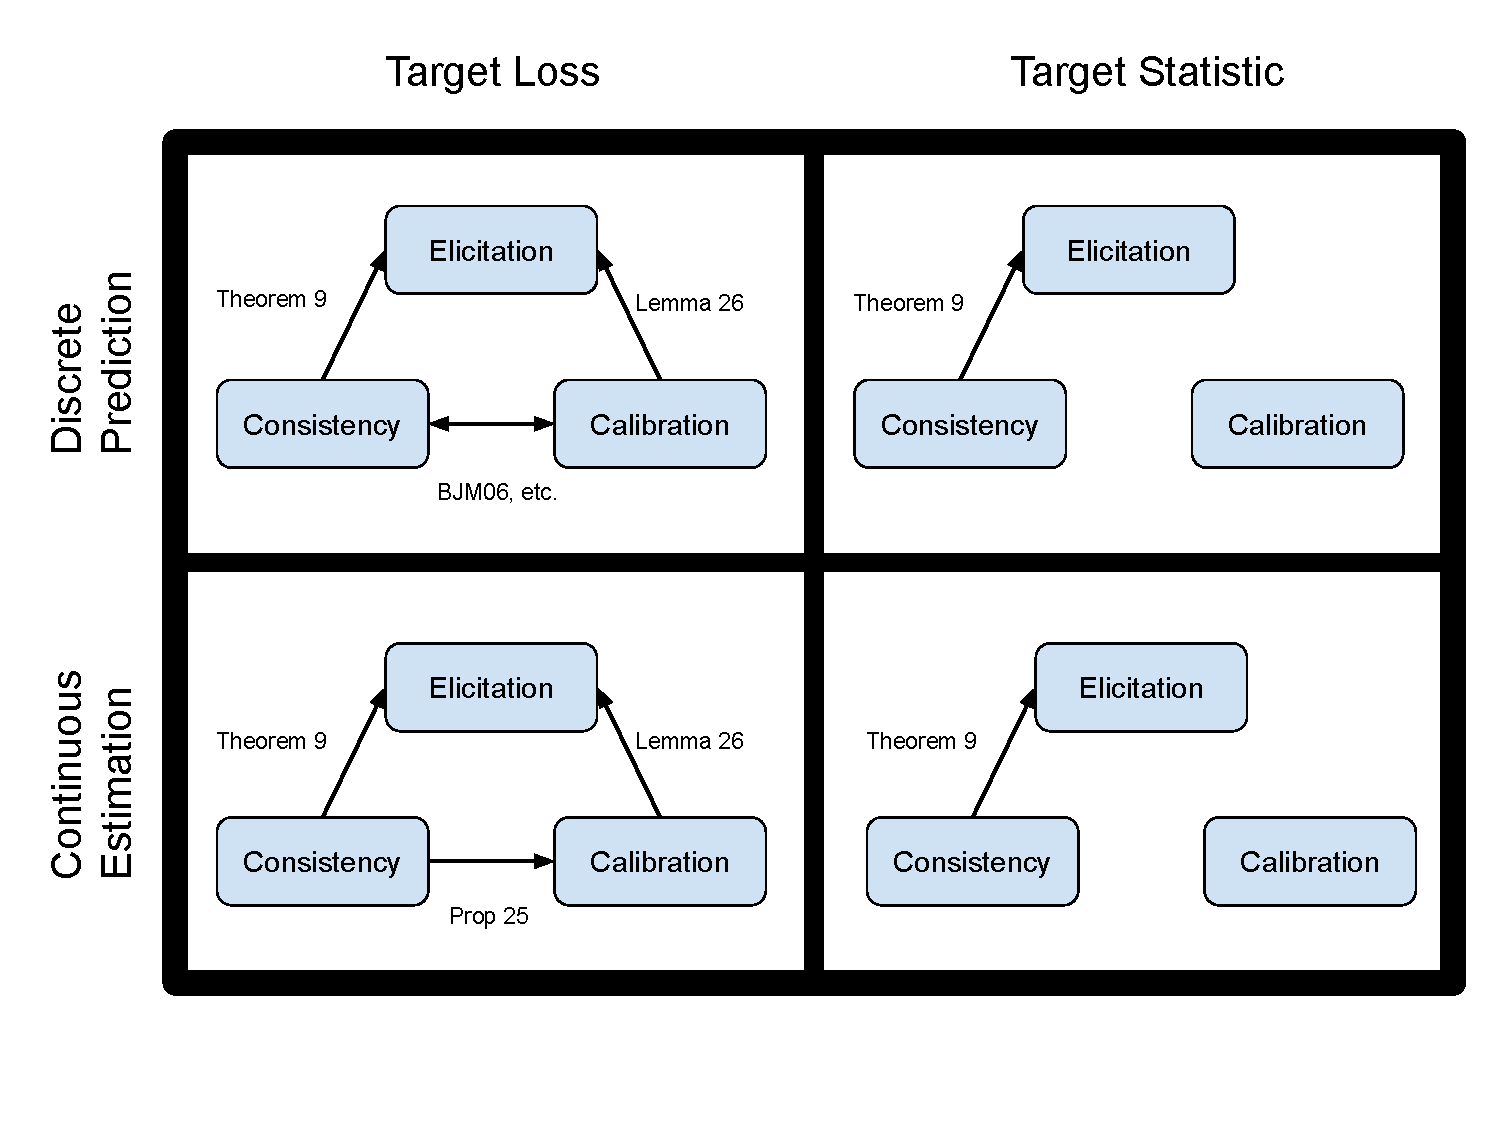
\includegraphics[width=0.95\linewidth]{tikz/consistency-elicitation-calibration.pdf}
%	\end{minipage}
%\end{figure}

% \begin{tabular}{lcccccl}\toprule
% & \multicolumn{3}{c}{$\tol=\tols$} & \multicolumn{3}{c}{$\tol=\told$}
% \\\cmidrule(lr){2-4}\cmidrule(lr){5-7}
%            & $mv$  & Rel.~err & Time    & $mv$  & Rel.~err & Time\\\midrule
% \trigmv    & 11034 & 1.3e-7 & 3.9 & 15846 & 2.7e-11 & 5.6 \\
% \trigexpmv & 21952 & 1.3e-7 & 6.2 & 31516 & 2.7e-11 & 8.8 \\
% \trigblock & 15883 & 5.2e-8 & 7.1 & 32023 & 1.1e-11 & 1.4e1\\
% \expleja   & 11180 & 8.0e-9 & 4.3 & 17348 & 1.5e-11 & 6.6 \\\bottomrule
% \end{tabular}

\begin{table}[t]
  \begin{center}
    \aboverulesep=1ex
    \belowrulesep=1ex
    \begin{tabular}{p{12ex}ll}
      & \emph{Target loss}  & \emph{Target statistic}\\
      \cmidrule[1pt]{2-3}
      \parbox{12ex}{\emph{Discrete \\ prediction}} & \textbf{Q1:} Classification  & \textbf{Q2:} Risk-averse classification\\ 
      \cmidrule{2-3}
      \parbox{12ex}{\emph{Continuous \\ estimation}} & \textbf{Q3:} Least-squares regression & \textbf{Q4:} Variance estimation\\ 
      \cmidrule[1pt]{2-3}
      \\
    \end{tabular}
    \caption{The four quadrants of problem types, with an example for each as discussed in \S~\ref{sec:illustration}.}
    \label{tab:quadrants}
  \end{center}
\end{table}

\begin{figure}[t]
\begin{center}
\resizebox{0.95\linewidth}{!}{%
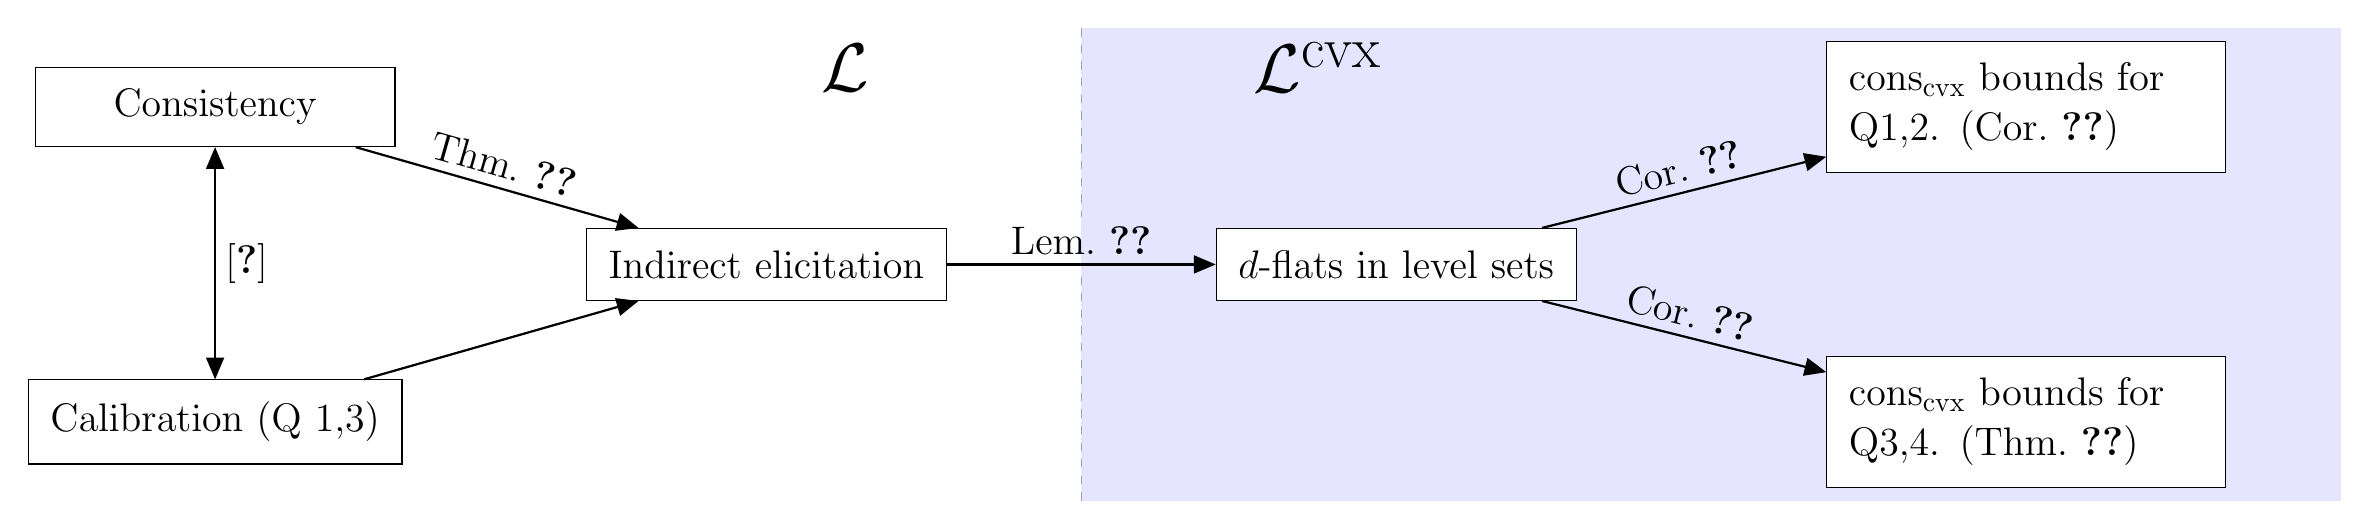
\begin{tikzpicture}

\tikzset{vertex/.style = {draw,minimum width=13em, inner sep=8pt, fill = white, font=\Large}}
\tikzset{edge/.style = {->,> = triangle 45, thick}}
\tikzset{node/.style = {anchor=above, sloped}}
\tikzstyle{every node}=[font=\Large]

\path[fill=blue, fill opacity = 0.1] (0,-3) -- (0,3) -- (16,3) -- (16,-3) -- cycle;
\draw[dashed, opacity = 0.3] (0,-3) -- (0,-0.1);
\draw[dashed, opacity = 0.3] (0,3) -- (0,0.6);
\node[draw=none] at (3,2.5) {{\Huge$\Lcvx$}};
\node[draw=none] at (-3,2.5) {{\Huge$\L$}};

% vertices
\node[vertex] (consistent) at  (-11,2) {Consistency};
\node[vertex] (calibrated) at  (-11,-2) {Calibration (Q 1,3)};
\node[vertex] (indir-elic) at  (-4,0) {Indirect elicitation};


\node[vertex] (d-flats) at  (4,0) {$d$-flats in level sets};
\node[vertex, text width=45mm] (q1-bounds) at (12,2) {$\conscvx$ bounds for Q1,2. (Cor.~\ref{cor:fsd-bound})};
\node[vertex, text width=45mm] (q4-bounds) at (12,-2) {$\conscvx$ bounds for Q3,4. (Thm.~\ref{thm:bayes-risk-lower-bound})};

%edges
\draw[edge, <->] (consistent) to node[right,text width=5mm]{\cite{bartlett2006convexity}} (calibrated);
\draw[edge] (consistent) to node[above, sloped]{Thm.~\ref{thm:consistent-implies-indir-elic}} (indir-elic);
\draw[edge] (calibrated) to (indir-elic);
\draw[edge] (indir-elic) to node[above, sloped]{Lem.~\ref{lem:convex-flats-inf-dim}} (d-flats);

\draw[edge] (d-flats) to node[above, sloped]{Cor.~\ref{cor:Pcodim-flat-elic-relint-prop}} (q4-bounds);
\draw[edge] (d-flats) to node[above, sloped]{Cor.~\ref{cor:Pcodim-flat-single-val-prop}} (q1-bounds);
\end{tikzpicture}
}
\end{center}
\caption{Flow and implications of our results. Compared to calibration, we suggest indirect elicitation as a simpler but almost-as-powerful necessary condition for consistency. In particular, we obtain a testable necessary condition, based on $d$-flats, for whether there exists a $d$-dimensional consistent convex surrogate. This condition recovers and strengthens existing calibration-based results.}
\label{fig:results-flow}
\end{figure}

\paragraph{Broader Impacts via influence on downstream research.}
\jessiet{Taken from original BI statement for this paper}
This paper takes a step toward an impactful general program: to understand and design \emph{useful} (i.e. convex, consistent, calibrated, etc.) surrogate losses of low dimensionality.
The theory in this paper may help practitioners in a number of ways.
Understanding how to design consistent convex surrogates for different target losses and properties we wish to learn, and when this is impossible, can lead to understanding the tradeoffs that are often made in the current ad-hoc design of surrogates.
These ad-hoc surrogates are consistent with respect to \emph{some property}, although it may not be the one we wish to elicit, either directly or indirectly.
As a general prediction task arises, one might be able to use property elicitation to understand what question they are actually answering (in the best case, with sufficient data that matches the real-world data distribution) by minimizing their surrogate loss and how it differs from the question they are actually trying to answer.
Of course, improvements in general machine learning algorithms can be put to many uses in many societal contexts, so a more specific analysis of potential broader impacts appears very difficult to forecast.

\section{Setting}\label{sec:related-work}

We consider supervised learning problems in the space $\X \times \Y$, for some \emph{feature space} $\X$ and a \emph{label space} $\Y$, with data drawn from a distribution $D$ over $\X \times \Y$.
The task is to produce a hypothesis $f: \X \to \R$, for some \emph{prediction space} $\R$, which may be different from $\Y$.
For example, in ranking problems, $\R$ may be all $|\Y|!$ permutations over the $|\Y|$ labels forming $\Y$.
As we focus on conditional distributions $p := D_x = \Pr[Y|X=x]$ over $\Y$ given some $x \in X$, we often abstract away $x$, working directly with a convex set of distributions over outcomes $\P \subseteq \simplex$.
We then write e.g.\ $\E_p L(\cdot,Y)$ to mean the expectation when $Y\sim p$.

If given, we use $\ell: \R \times \Y \to \reals$ to denote a \emph{target loss}, with predictions $r\in\R$.
%where the goal is minimize expected loss, $\E ~ \ell(f(X),Y)$ for pairs $X,Y$ drawn from some distribution.
Similarly, $L: \reals^d \times \Y \to \reals$ will typically denote a \emph{surrogate} loss, with surrogate predictions $u \in \reals^d$.
We write $\L_d $ for the set of $\mathcal{B}(\reals^d) \otimes \Y$-measurable and lower semi-continuous surrogates $L : \reals^d \times\Y \to \reals$ such that $\E_{Y \sim p} L(u,Y) < \infty$ for all $u \in \reals^d, p \in \P$, that are minimizable in that $\argmin_{u} \exploss{L}{u}{p}$ is nonempty for all $p\in\P$.
Moreover, $\Lcvx_d \subseteq \L_d$ is the set of convex (in $\reals^d$ for every $y \in \Y$) losses in $\L_d$.
\btw{Sufficient condition for $\A$-normal convex integrand: $L$ is lower semi-continuous and $\mathcal{B}(\A) \otimes \Y$-measurable; $\E_p L(u,Y)$ finite for all $u, p$, there exists a $u_0$ for each $p$ so that $\E_p L(u_0, Y)$ is finite and continuous for Rockefellar's corollary, though it's stricter than Ioffe and Tokhimorov IIRC}
%Similarly, let $\L_d^{fin}$ be surrogates $L: \reals^d \times \Y \to \reals$ that are $\mathcal{B}(\reals^d) \otimes \Y$-measurable and minimizable, in the sense that $\argmin_{u} \exploss{L}{u}{p}$ is nonempty for all $p\in\P$-- we use this class of losses with finite $\Y$ in mind.
Set $\L = \cup_{d \in \mathbb{N}} \L_d$, and $\Lcvx = \cup_{d \in \mathbb{N}} \Lcvx_d$.
A loss $\ell: \R\times \Y \to \reals$ is \emph{discrete} if $\R$ is a finite set.
%A surrogate $L:\reals^d \times \Y \to \reals$ is \emph{convex} if $L(\cdot,y)$ is convex in $u$ almost surely in $\Y$.
\jessiet{Need this?}
\raft{Assuming you mean regret -- no I think we can move to the appendix now, for consistency stuff}
For a given $p\in\P$, the (conditional) \emph{regret}, or excess risk, of a loss $L$ is given by $R_L(u,p) := \exploss{L}{u}{p} - \inf_{u^*} \exploss{L}{u^*}{p}$.
Typically, we notate finite report sets $\R$.


% For a distribution $p \in \simplex$, we denote the expected target loss for prediction $r$ to be $\E_{Y \sim p} \ell(r, Y) := \ell(r; p)$.
% Similarly, $\E_{Y \sim p} L(u, Y) := L(u ; p)$.






\subsection{Property elicitation}\label{subsec:properties}
\jessiet{This sentence might make me wary of minnability assumptions as a reviewer}
\raft{True, but we address it below.  We could forward reference that discussion.  I think it's okay though.}
Arising from the statistics and economics literature, property elicitation is similar to calibration, but only characterizes exact minimizers of a surrogate~\citep{savage1971elicitation,osband1985information-eliciting,lambert2008eliciting,lambert2009eliciting,lambert2018elicitation,frongillo2015vector-valued,frongillo2014general}.
Specifically, given a statistic or \emph{property} $\Gamma$ of interest, which maps a distribution $p \in \P \subseteq \simplex$ to the set of desired or correct predictions, the minimizers of $L$ should precisely coincide with $\Gamma$.
For example, squared loss $L(r,y) = (r-y)^2$ elicits the mean $\Gamma(p) = \E_p Y$.
For intuition, to relate to consistency, one can think of $p = \Pr[Y|X=x]$ as a conditional distribution, though the definition is also applied to point prediction settings.

\begin{definition}[Property, elicits]
	A \emph{property} is a set-valued function $\Gamma : \P \to 2^\R \setminus \{\emptyset\}$, which we denote $\Gamma: \P \toto \R$.
	A loss $L : \R \times \Y \to \reals$ \emph{elicits} the property $\Gamma$ if
	\begin{equation}
    \label{eq:elic}    
    \forall p \in \P, \;\; \Gamma(p) = \argmin_{u \in \R} \exploss{L}{u}{p}~.
	\end{equation}
\end{definition}
An example is the mean, $\Gamma(p) = \{\E_p Y\}$.
The \emph{level set} of $\Gamma$ at value $r\in\R$ is $\Gamma_r := \{p \in \P : r \in \Gamma(p)\}$.
We call a property $\Gamma: \P \toto \R$ \emph{discrete} if $\R$ is a finite set, as in Quadrants 1 and 2.
A property is \emph{single-valued} if $|\Gamma(p)|=1$ for all $p\in\P$, in which case we may write $\Gamma:\P\to\R$ and $\Gamma(p) \in \R$.
As an example, the mean is single-valued.
We define the \emph{range} of a property by $\range \Gamma = \bigcup_{p\in\P} \Gamma(p) \subseteq \R$.
When $L\in\L$, we use $\Gamma := \prop[\P]{L}$ to denote the unique property elicited by $L$ (for distributions in $\P$) from eq.~\eqref{eq:elic}. 
Typically, we denote the target property by $\gamma$, and the surrogate by $\Gamma$.

To relate property elicitation to consistency, we need to allow for a link function, which gives rise to the notion of \emph{indirect} elicitation.
For single-valued properties, this definition reduces to the natural requirement $\gamma = \psi \circ \Gamma$.
\begin{definition}[Indirect Elicitation]\label{def:indirectly-elicits}
	A surrogate loss and link $(L, \psi)$ \emph{indirectly elicit} a property $\gamma:\P \toto \R$ if $L$ elicits a property $\Gamma: \P \toto \reals^d$ such that for all $u \in \reals^d$, we have $\Gamma_u \subseteq \gamma_{\psi(u)}$.
	We say $L$ \emph{indirectly elicits} $\gamma$ if such a link $\psi$ exists.
  \btw{interesting discussion of set-valued properties commented out; revive later!}
\end{definition}

As observed implicitly and explicitly in the literature, e.g.~\citep{steinwart2008support,agarwal2015consistent}, the following proposition states that consistency implies indirect elicitation.
Informally, consistency means that a hypothesis sequence converging to the optimal surrogate loss, in expectation over the data distribution $\D \sim \X \times \Y$, links to a sequence converging to the optimal target loss or conditional statistical value.
See \S~\ref{sec:consis-implies-indir} for definitions and the proof.

\begin{restatable}{proposition}{consistencyimpliesindirelic}\label{thm:consistent-implies-indir-elic}
	For a surrogate $L \in \L$, if the pair $(L, \psi)$ is consistent with respect to a property $\gamma: \P \toto \R$ or a loss $\ell$ eliciting $\gamma$, then $(L, \psi)$ indirectly elicits $\gamma$.
\end{restatable}

% While there are several possible set-valued extensions, Definition~\ref{def:indirectly-elicits} best matches  suited for studying consistency.
% There are a few possible definitions of indirect elicitation, but this is the most applicable for our setting because when we consider set-valued properties, we do not have that \emph{all} optimal predictions for $\Gamma$ must be linked back to \emph{all} optimal predictions for $\gamma$.
% Instead, we lighten this restriction to say that any optimal prediction for $\Gamma$ must be linked to \emph{an} optimal prediction for $\gamma$, and we must do so deterministically. 

Implicit in the above elicitation definitions is that $L\in\L$, meaning $L$ is minimizable: since $\Gamma = \prop[\P]{L}$ is nonempty everywhere, the expected loss $\exploss{L}{\cdot}{p}$ always achieves a minimum.
This restriction is also implicit in previous work, e.g.,~\citep{agarwal2015consistent}.
While some popular surrogates such as logistic and exponential loss are not minimizable, these losses are still covered in Corollary~\ref{cor:Pcodim-flat-elic-relint-prop} and Theorem~\ref{thm:bayes-risk-lower-bound} as $\Gamma(p) \neq \emptyset$ when $p\in\P := \relint\simplex$; moreover, by thresholding $L'(u,y) = \max(L(u,y),\epsilon)$ for sufficiently small $\epsilon>0$ we can achieve $L'\in\L$ for both.
We expect that a generalization of property elicitation which allows for ``infinite'' predictions (e.g., along a prescribed ray) would allow us to assume minimizability without loss of generality, as convex losses would always admit this more general minimizer.
\btw{Some refs / related work commented out here.  I think not as relevant as elicitation complexity.}

% Property elicitation of a single property is well-understood~\citep{savage1971elicitation,osband1985information-eliciting,lambert2008eliciting, lambert2009eliciting, lambert2018elicitation}, and \citet{finocchiaro2018convex} are among the first to consider \emph{convex} elicitable properties.
% Additionally, \citet{agarwal2015consistent} are the first to our knowledge to formally relate property elicitation to the consistency of a surrogate loss, although they only consider settings with $|\Y| < \infty$. \jessiet{right?}
%However, their assumptions are more restrictive than ours; they only consider losses defined on the real line.% and assume the properties to be identifiable: an assumption we do not need.


\subsection{Convex consistency dimension and elicitation complexity}\label{subsec:complexity}

Various works have studied the minimum prediction dimension $d$ needed in order to construct a consistent surrogate loss $L: \reals^d \times \Y \to \reals$, typically through proxies such as calibration~\citep{steinwart2008support,agarwal2015consistent,ramaswamy2016convex} and property elicitation~\citep{frongillo2015vector-valued,fissler2016higher,frongillo2020elicitation}.
In Quadrant 1, \citet{ramaswamy2016convex} introduce a special case of convex consistency dimension (Definition~\ref{def:cvx-consistency-dim}), which led to consistent convex surrogates for discrete prediction problems such as hierarchical classification~\citep{ramaswamy2015hierarchical} and classification with an abstain option~\citep{ramaswamy2018consistent}.

%\raft{FYI Jessie: Two general points.  (1) I spent the majority of my time in this section just on dependencies; e.g.\ you had ``similar to elicitation complexity mentioned above'' but elicitation complexity was not mentioned above.  Next time it would be more efficient if you made sure to balance local edits with global scans to catch these sorts of things, as well as making sure we aren't explaining things twice, etc.  (2) You tend to mix background with nods to our results, which is actually good to do, but it can be jarring if you go back and forth too much.  See for example how I changed the previous subsection, reserving the nod to our work to the end of the subsection.}\jessiet{Noted boss man}

%\begin{definition}[Convex Calibration Dimension]
%	Given a target discrete loss $\ell$, its \emph{convex calibration dimension} $\ccdim(\ell)$ is the minimum dimension $d$ such that there is a $L \in \Lcvx_d$ and link $\psi$ such that $(L,\psi)$ is calibrated with respect to $\ell$.
%	jessiet{Change this def to be about consistent prediction dimension}
%  \btw{Maybe take out of definition environment, but (a) I'd worry that people wouldn't be able to find the definition when we use it later, and (b) I'm hoping we can make the distinction very clear, which now is achieved by the parallel definitions}
%\end{definition}

\begin{definition}[Convex Consistency Dimension]\label{def:cvx-consistency-dim}
  Given target loss $\ell:\R \times\Y \to \reals$ or property $\gamma: \P \toto \R$, its \emph{convex consistency dimension} $\conscvx(\cdot)$ is the minimum dimension $d$ such that $\exists L \in \Lcvx_d$ and link $\psi$ such that $(L,\psi)$ is consistent with respect to $\ell$ or $\gamma$.
%	\btw{Maybe take out of definition environment, but (a) I'd worry that people wouldn't be able to find the definition when we use it later, and (b) I'm hoping we can make the distinction very clear, which now is achieved by the parallel definitions}
\end{definition}
% \jessiet{Cut this sentence?  Lots of refs to it}
% \emph{Consistency} is defined for a target loss in Definition~\ref{def:consistent-ell} and for a target property in Definition~\ref{def:consistent-prop} in Appendix~\ref{sec:consis-implies-indir}.

In the case of a target property $\gamma$, i.e. a statistic, \citet{lambert2008eliciting} similarly introduce the notion of \emph{elicitation complexity}, later generalized by \citet{frongillo2020elicitation}, which captures the lowest prediction dimension of a surrogate which indirectly elicits $\gamma$.
This notion is quite general as it includes continuous estimation settings and does not inherently depend on a target loss being given. 
% However, until now, no formal connection to consistency has been shown for convex elicitation complexity.

\begin{definition}[Convex Elicitation Complexity]\label{def:cvx-elic-complex}
	Given a target property $\gamma$, the \emph{convex elicitation complexity} $\eliccvx(\gamma)$ is the minimum dimension $d$ such that there is a $L \in \Lcvx_d$ indirectly eliciting $\gamma$.
\end{definition}

\begin{corollary}\label{cor:elic-lb-consis-dim}
	Given a property $\gamma : \P \toto \R$ or loss $\ell:\R \times \Y \to \reals$ eliciting $\gamma$, we have $\eliccvx(\gamma) \leq \conscvx(\gamma) = \conscvx(\ell)$.
\end{corollary}

%As we show next, calibration implies indirect elicitation, which means the convex elicitation complexity always lower bounds the convex calibration dimension in the setting of discrete target losses.
%Yet despite this fact, the state-of-the-art lower bound for convex calibration dimension, the \emph{feasible subspace dimension} of \citet{ramaswamy2016convex}, is a special case of our lower bound for convex elicitation complexity (Theorem~\ref{thm:cvx-flats}), meaning we achieve the same or even higher lower bounds.
%(See the examples in \S~\ref{subsec:examples-finite}.)
%Moreover, convex elicitation complexity also applies beyond the discrete target loss setting, as we demonstrate in \S~\ref{sec:contin-consis}.

\citet[Corollary 10]{agarwal2015consistent} provide a necessary condition for the direct convex elicitation of single-valued properties, yielding bounds on the dimensionality of level sets.
Moreover, \citet{finocchiaro2019embedding} study surrogate losses which \emph{embed} a discrete loss, which is a special case of indirect elicitation.
%They construct calibrated link functions from embeddings, which together with observations about indirect elicitation, imply that for polyhedral (piecewise linear and convex) losses, calibration and indirect elicitation are equivalent.
\citet{finocchiaro2020embedding} further introduce the notion of \emph{embedding dimension}, which is a lower bound on both convex elicitation complexity of discrete properties and convex consistency dimension of discrete losses and finite statistics.
%\btw{Bo: commented out what I felt was an unnecessary sentence}
%Since embedding is a special case of indirect elicitation, we have the chain of inequalities, embedding dimension $\leq$  ``polyhedral calibration dimension'' $\leq$ convex calibration dimension; it is an open problem whether any of these inequalities can be strict.




\section{Prediction Dimension of Consistent Convex Surrogates}\label{sec:char-convex}
We now turn to the question of bounding the prediction dimension of a consistent convex surrogate.
From Theorem\jessie{Proposition} \ref{thm:consistent-implies-indir-elic} in Appendix~\ref{sec:consis-implies-indir}, given a target property $\gamma$ or loss $\ell$ with $\gamma = \prop{\ell}$, this task reduces to lower bounding the prediction dimension of a convex surrogate indirectly eliciting $\gamma$.
%We now explore two tools, Corollaries~\ref{cor:Pcodim-flat-single-val-prop} and~\ref{cor:Pcodim-flat-elic-relint-prop}, for proving such convex elicitation lower bounds.
Lemma~\ref{lem:convex-flats-inf-dim}, crystallized from the proofs of \citet[Theorem 16]{ramaswamy2016convex} and \citet[Theorem 9]{agarwal2015consistent}, considers a particular distribution~$p$ and surrogate prediction $u \in \reals^d$ with is optimal for $p$.
Lemma~\ref{lem:convex-flats-inf-dim} will show that if $d$ is small, then the level set $\{p \in \P : u \in \argmin_{u'} \exploss{L}{u'}{p}\}$ must be large; in fact, it must roughly contain a high-dimensional \emph{flat}.
By definition of indirect elicitation, there is some level set $\gamma_r$ (where $u$ is linked to $r$) containing this flat as well.
The use of this result is to leverage the contrapositive: if $\gamma$ has a level set intricate enough to not contain any high-dimensional flats, then $\gamma$ cannot have a low-dimensional consistent surrogate.

%Recall $\affhull(\simplex) = \{\sum_{i=1}^n \alpha_i p_i : p_i \in \simplex, \alpha_i \in \reals, \sum_{i=1}^n \alpha_i = 1\}$, which has dimension $n-1$.
%Moreover, $\ker(W) = \{p \in \spn(\P): Wp = \vec 0\}$ is the kernel of matrix $W$.
%Recall that the affine hull is the set of all linear combinations whose coefficients sum to 1.
%In particular, we will often use \footnote{Recall $\affhull(\simplex) = \{\sum_{i=1}^n \alpha_i p_i : p_i \in \simplex, \alpha_i \in \reals, \sum_{i=1}^n \alpha_i = 1\}$, which has dimension $n-1$.}\jessiet{Space suggestion: move terse version of this to footnote.}

\begin{definition}[$d$-flat]\label{def:flat-general}
  For $d\in\mathbb N$, a \emph{$d$-flat}, or simply \emph{flat}, is a nonempty set $F = \zeros{W} := \{q \in \P : \E_q W = \vec 0\}$ for some measurable $W:\Y \to \reals^d$.
\end{definition}

The following Lemma yields Corollaries~\ref{cor:Pcodim-flat-single-val-prop} and~\ref{cor:Pcodim-flat-elic-relint-prop} (in Appendix~\ref{app:implications-of-bounds}), which when combined with Theorem\jessie{prop?} \ref{thm:consistent-implies-indir-elic}, yield consistency bounds.
A similar result is found in \citet[Theorem 9]{agarwal2015consistent}, which bounds the dimension of level sets of a single-valued $\prop{L}$.
Lemma~\ref{lem:convex-flats-inf-dim} instead bounds the dimension of flats contained in the level sets, an additional power which we leverage in our examples.


\begin{lemma}
  \label{lem:convex-flats-inf-dim}
  Let $\Gamma:\P \toto \reals^d$ be (directly) elicited by $L \in \Lcvx_d$ for some $d\in\mathbb{N}$.
  Let $\Y$ be either a finite set, or $\Y = \reals$, in which case we assume each $p\in\P$ admits a Lebesgue density supported on the same set for all $p\in\P$.%
  \footnote{This assumption is largely for technical convenience, to ensure that $\V_{u,p}$ does not depend on $p$.
    Any such assumption would suffice, and we suspect even that condition can be relaxed.}
  For all $u\in\range\Gamma$ and $p\in\Gamma_u$, there is some $V_{u,p}:\Y\to\reals^d$ such that $p \in \zeros{V_{u,p}} \subseteq \Gamma_u$.
  \jessie{Change back to Theorem}
\end{lemma}
\begin{proof}
  As $L$ is convex and elicits $\Gamma$, we have $u \in \Gamma(p) \iff \vec 0 \in \partial \exploss{L}{u}{p}$. 
  We proceed in two cases, depending on $|\Y|$.
  
  \emph{Finite $\Y$: }
  If $\Y$ is finite, this is additionally equivalent to $\vec 0 \in \oplus_y p_y \partial L(u,y)$, where $\oplus$ denotes the Minkowski sum~\citep[Theorem 4.1.1]{hiriart2012fundamentals}.\footnote{$\partial$ represents the subdifferential $\partial f(x) = \{z : f(x') - f(x) \geq \inprod{z}{x'-x}\; \forall x' \}$.}
  Expanding, we have $\oplus_y p_y \partial L(u,y) = \{ \sum_{y\in\Y} p_y x_y \mid x_y \in \partial L(u,y) \; \forall y\in\Y\}$, and thus $W p = \sum_y p_y x_y = \vec 0$ where $W = [x_1, \ldots, x_n] \in \reals^{d\times n}$; cf.~\cite[$\mathbf{A}^m$ in Theorem 16]{ramaswamy2016convex}.
  Let $V_{u,p} : \Y \to \reals^d, y \mapsto W_y$ be the function encoding the columns of $W$.
  Observe that $\E_p V_{u,p} = \vec 0$.				
  
  \emph{$\Y=\reals$: }
  \btw{Note: this should work for any infinite $\Y$ so long as you have a good $\sigma$-algebra... working at least with $\Y \subseteq \reals$ just makes things easier since we can take the Borel $\sigma$-algebra for granted.}
  Any $L \in \Lcvx_d$ satisfies the assumptions of~\cite{ioffe1969minimization}, so we may interchange subdifferentiation and expectation.
  Specifically, letting $\V_{u,p} = \{V:\Y\to\reals^d \mid V \text{ measurable}, V(y) \in \partial L(u,y) \text{ $p$-a.s.}\}$, we have
  $\partial \E_p L(u,Y) = \{\int V(y)dp(y) \mid V\in\V_{u,p}\}$.
  As $\vec 0 \in \partial \E_p L(u,Y)$, in particular, there is some $V_{u,p} \in \V_{u,p}$ such that $\E_p V_{u,p} = 0$.
  \btw{Fleshing this out: $\exists E \subseteq \mathcal{B}(\Y)$ so that $p(E) = 0$ and $V(y) \in \partial L(u,y) \forall y \in E^c$.  Claim $q(E) = 0$, which would complete the claim that $V(y) \in \partial L(u,y) q$-a.s.  For contradiction, if $q(E) > 0$, then $\exists x \in E$ and open neighborhood $N_x \ni x$ with $q(N_x) > 0$.  Since $\supp(p) = \supp(q)$, we then have $p(N_x) >0$, contradicting $p(E) = 0$, and hence $V(y) \in \partial L(u,y)$ not $p$-a.s.  Therefore, we must have $q(E) = 0$, so $V(y) \in \partial L(u,y) q$-a.s.}
  For any $q\in\P$, as by assumption $q$ is supported on the same set as $p$, we have $V_{u,p}(y)\in\partial L(u,y)$ $q$-a.s., so that $V_{u,p}\in\V_{u,q}$\btw{I'm a bit too tired to see exactly how this follows, but it seems intuitively obvious. I'm okay to punt on it for the submission, but if someone has time to check, that would be great! \jessie{See above margin comment.  I think it's too much detail for the conference submission, but feel free to change my mind.}}.
  Thus, $\E_q V_{u,p} = 0$ implies $0\in\partial\E_q L(u,Y)$ by the above.
  \btw{For posterity, the bug: we want to conclude $\E_q V_{u,p} = 0 \implies q \in \Gamma_u$.  But the ``a.s.\ in $p$'' means we may not have $0 \in \partial \E_q L(u,Y)$, since maybe $V_{u,p}(y)$ is not in $\partial L(u,y)$ a.s.\ in $q$...}
  
  In both cases, we take the flat $F := \zeros{V_{u,p}}$, and have $p \in F$ by construction.
  To see $F \subseteq \Gamma_u$, from the chain of equivalences above, we have for any $q\in\P$ that $q \in \zeros{V_{u,p}} \implies \vec 0 \in \partial \E_q L(u,Y) \implies u \in \Gamma(q) \implies q \in \Gamma_u$.
\end{proof}

%Knowing indirect elicitation implies the existence of such a flat, we now apply  Theorem~\ref{thm:consistent-implies-indir-elic} and Lemma~\ref{lem:convex-flats-inf-dim} to construct lower bounds on convex consistency dimension.

%\begin{lemma}
%	Let $\gamma$ be indirectly elicited by some $d$-convex-elicitable $\Gamma$ for $d\in\mathbb{N}$.
%	For all $r\in\range\gamma$ and $p$ such that $|\gamma(p)| = 1$ with $\{r\} = \gamma(p)$, there is some flat $F$ \jessie{of \Pcodimension at most $d$?} such that $p \in F \subseteq \gamma_r$.
%\end{lemma}



\subsection{Illustration: geometric intuition for the four quadrants}
\label{sec:illustration}
We can apply Lemma~\ref{lem:convex-flats-inf-dim} to construct lower bounds on convex consistency dimension for targets across all four quadrants by Corollaries~\ref{cor:Pcodim-flat-single-val-prop} (for continuous estimation problems; Q3, Q4) and~\ref{cor:Pcodim-flat-elic-relint-prop} (for discrete prediction problems; Q1, Q2).
The illustrations in Table~\ref{tab:quadrants-simplices} are simply intended to show how Lemma~\ref{lem:convex-flats-inf-dim} can be applied to results in all four quadrants of problem types-- making it the first lower bound to our knowledge to do so.

\paragraph{Q1: Abstain}
The abstain target loss is a well-studied variation of 0-1 loss that allows for an ``abstain'' report that gives a lesser punishment $1/2$ for abstaining, $r = \bot$.
Given the target loss $\ell^{1/2}(r,y) := \Ind{r \not \in \{y, \bot\}} + (1/2)\Ind{r = \bot}$,  we can consider the \emph{abstain property} $\gamma$ it elicits, where one predicts the most likely outcome $y$ if $Pr[Y=y|x] \geq 1/2$ and ``abstain'' by predicting $\bot$ otherwise.
Since we are given a discrete target loss, this problem fits nicely into Quadrant 1.

When $n =3$, the property $\gamma^{1/2}$ elicited by $\ell^{1/2}$ is depicted in Table~\ref{tab:quadrants-simplices} (Q1).
Upon closer inspection, the level set boundaries are found at the set of distribution where is a $y$ such that $p_y = 1/2$.
For any distribution $p \in \relint{\gamma_\bot}$, we can derive a lower bound on convex consistency dimension by trying to fit a $1$-flat through this point; however, by the global geometry of the property and location of the abstain cell relative to other cells, we cannot fit a $1$-flat (line in the 2-d projection of the simplex here) fully contained in $\gamma_\bot$ that passes through $p = \bullet$.
By Corollary~\ref{cor:Pcodim-flat-elic-relint-prop}, we can conclude $\conscvx(\gamma^{1/2}) \geq 2$ over $3$ outcomes.
\citet{ramaswamy2016convex} present a convex surrogate for the abstain loss yielding a logarithmic upper bound on $\conscvx(\ell^{1/2})$, so this bound is tight.% which are an exponential improvement over previous results, e.g.,~\citep{crammer2001algorithmic,rifkin2004defense}.

\paragraph{Q2: High confidence classification}
Consider the following scenario where someone is deciding how to dress for the weather based on a meteorologist's forecast: a forecaster is choosing between three outcomes $\Y = \{$rainy, sunny, snowy$\}$, and we suppose we want to have some bias towards health and safety, so the meteorologist should only predict sunny weather if $Pr[$sunny $|$ weather data$] \geq 3/4$.
Otherwise, they should predict whatever is more likely  given the weather data: rain or snow.

We can now model this problem by a property with the reports $\R = \Y$, and have 
\begin{align*}
\gamma(p) &= \begin{cases}
\text{sunny} & p_{\text{sunny}} \geq 1/2 \\
\text{rainy} & p_{\text{sunny}} \leq 1/2 \wedge p_{\text{rainy}} \geq p_{\text{snowy}} \\
\text{snowy} & p_{\text{sunny}} \leq 1/2 \wedge p_{\text{snowy}} \geq p_{\text{rainy}} \\
\end{cases}~,~
\end{align*} 

This property is shown in Table~\ref{tab:quadrants-simplices} (Q2), and we can observe the point $p = \bullet = (0.3,0.3,0.4)$ that, like abstain, we cannot fit a $1$-flat entirely contained in the level set $\gamma_{\text{snowy}}$ through $p$.
Therefore, we can apply Corollary~\ref{cor:Pcodim-flat-single-val-prop} to conclude that $\conscvx(\gamma) = 2$.

\paragraph{Q3: Least-squares regression}
\jessie{Define property, discuss briefly why in the quadrant.  Move to how results apply and what they say}
While least squares regression is commonly used in machine learning and statistics for continuous estimation, it might not be immediately \emph{why} we do so, prompting us to study this smooth convex loss in Quadrant 3.
Evaluating the derivative of squared loss, we can observe that it elicits the expected value $\Gamma(p) = \E_p[Y]$.
With $\Y = \{-1,0,1\}$, we can visualize the level sets of the expected value as in Table~\ref{tab:quadrants-simplices} (Q3).
Since squared loss is a $1$-dimensional loss, we can verify that for all $p \in \simplex$, we can fit a $1$-flat (precisely equal to the level set) through $p$, as demonstrated in the Table.

\paragraph{Q4: Variance}
In understanding uncertainty, one might reasonably want to estimate the variance $\Gamma^\Var(p) = \E_p[Y^2] - \E_p[Y]^2$.
This property is continuous in the simplex $\simplex$, and therefore belongs in Quadrant 4.
The well-known fact that the variance is not elicitable does not yield a lower bound on elicitation complexity of 2, as it does not rule out the variance being a link of a real-valued convex-elicitable property; cf.~\citet[Remark 1]{frongillo2020elicitation}.
However, in Appendix~\ref{app:omitted-examples}, we show $\eliccvx(\Gamma^\Var)=2$, meaning the lowest dimension of a convex loss to estimate conditional variance is 2. %~\citep{osband1985providing,lambert2018elicitation}.
This lower bound will follow from Theorem~\ref{thm:bayes-risk-lower-bound} using the fact that variance is the Bayes risk of squared loss $L(r,y) = (r-y)^2$, which elicits the mean $\Gamma(p) = \E_p Y$.
Interestingly, while perhaps intuitively obvious, even this simple result is novel.

\begin{SCtable}
\begin{tabular}{c|c}
	%\hline
	\begin{tikzpicture} [scale=\tikzfigscale, thick, tdplot_main_coords]
	% standard tikz coordinate definition using x, y, z coords
	\coordinate (orig) at (0,0,0);
	
	\pgfmathsetmacro{\ph}{0.54}
	\pgfmathsetmacro{\pm}{0.23}
	\pgfmathsetmacro{\pl}{0.23}
	\coordinate (p) at (\ph,\pm,\pl);
	\coordinate (uniform) at (1/3,1/3,1/3);
	\coordinate[label=below:${y_1}$] (h) at (1,0,0);
	\coordinate[label=below:${y_3}$] (m) at (0,1,0);
	\coordinate[label=right:${y_2}$] (l) at (0,0,1);
	
	% draw axes
	\draw[simplex] (h) -- (m) -- (l) -- (h);
	
	\begin{scope}
	\clip (h) -- (m) -- (l) -- (h);
	\draw[myblue] (1/2,1/2,0) -- (1/2, 0, 1/2);
	\draw[myblue] (0,1/2,1/2) -- (1/2, 0, 1/2);
	\draw[myblue] (0,1/2,1/2) -- (1/2,1/2, 0);
	\coordinate (point) at (0.3,0.4, 0.3);
	\draw[orange, dashed,shorten >= -3cm, shorten <=-3cm] (1/4,3/4,0) -- (point);
	\draw[orange, dashed,shorten >= -3cm, shorten <=-3cm] (0.7,0,0.3) -- (point);
	\node at (point) {$\bullet$};
	%\draw[orange, very thick] (0.7,0.3,0) -- (0.7,0.3,2);
	\end{scope}
	\node[inner sep=2pt] (levset1) at (3/4,1/8,1/8) {$\gamma_{y_1}\!\!$};
	\node[inner sep=2pt] (levsetabs) at (5/12,5/12,1/6) {$\gamma_{\bot}$};
	%\draw[-latex,thin] (levset2) edge[in=270,out=90] (0.7,0.3,0);
	%\draw[-latex,thin] (levset1) edge[in=270,out=90] (0.3,0.7,0);
	\placefiglabel{(Q1)}
	\end{tikzpicture}
	&
	\begin{tikzpicture} [scale=\tikzfigscale, thick, tdplot_main_coords]
	% standard tikz coordinate definition using x, y, z coords
	\coordinate (orig) at (0,0,0);
	
	\pgfmathsetmacro{\ph}{0.54}
	\pgfmathsetmacro{\pm}{0.23}
	\pgfmathsetmacro{\pl}{0.23}
	\coordinate (p) at (\ph,\pm,\pl);
	\coordinate (uniform) at (1/3,1/3,1/3);
	\coordinate[label=below:${\text{rainy}}$] (h) at (1,0,0);
	\coordinate[label=below:${\text{sunny}}$] (m) at (0,1,0);
	\coordinate[label=right:${\text{snowy}}$] (l) at (0,0,1);
	
	% draw axes
	\draw[simplex] (h) -- (m) -- (l) -- (h);
	
	\begin{scope}
	\clip (h) -- (m) -- (l) -- (h);
	\draw[myblue,thick] (1/2,0,1/2) -- (0,1/2, 1/2);
	\def\e{1/16};
	\draw[myblue,thick] (1/4,1/4,1/2) -- (1/2, 1/2, 0);
	\coordinate (point) at (0.3,0.4, 0.3);
	\draw[orange, dashed,shorten >= -3cm, shorten <=-3cm] (0.4, 0.6, 0.) -- (point);
	\draw[orange, dashed,shorten >= -3cm, shorten <=-3cm] (0,0.4,0.6) -- (point);
	\node at (point) {$\bullet$};
	%\draw[orange, very thick] (0.3,0.7,0) -- (0.3,0.7,2);
	%\draw[orange, very thick] (0.7,0.3,0) -- (0.7,0.3,2);
	\end{scope}
	\node[inner sep=2pt] (levsetmin1) at (2/3, 1/6,1/6) {$\gamma_{\text{rainy}}$};
	\node[inner sep=2pt] (levset1) at (1/6,2/3,1/6) {$\gamma_{\text{snowy}}$};
	%\draw[-latex,thin] (levset2) edge[in=270,out=90] (0.7,0.3,0);
	%\draw[-latex,thin] (levset1) edge[in=270,out=90] (0.3,0.7,0);
	\placefiglabel{(Q2)}
	\end{tikzpicture}
	\\
	\hline
  \begin{tikzpicture} [scale=\tikzfigscale, thick, tdplot_main_coords]
% standard tikz coordinate definition using x, y, z coords
\coordinate (orig) at (0,0,0);

\pgfmathsetmacro{\ph}{0.54}
\pgfmathsetmacro{\pm}{0.23}
\pgfmathsetmacro{\pl}{0.23}
\coordinate (p) at (\ph,\pm,\pl);
\coordinate[label=below:${y=-1\!\!\!\!}$] (h) at (1,0,0);
\coordinate[label=below:${y=1}$] (m) at (0,1,0);
\coordinate[label=right:${y=0}$] (l) at (0,0,1);

% draw axes
\draw[simplex] (h) -- (m) -- (l) -- (h);

\begin{scope}
\clip (h) -- (m) -- (l) -- (h);
\foreach \c in {0,0.05,...,1}
{
	\pgfmathsetmacro\aa{\c}
	\coordinate (A) at ($(\aa,1-\aa,0)$);
	\coordinate (B) at ($(\aa,1-\aa,2)$);
	\draw[myblue,thin] (A) -- (B);
}
\draw[orange, thick,dashed] (0.45,0.55,0) -- (0.45,.55,2);
%\draw[orange, very thick] (0.7,0.3,0) -- (0.7,0.3,2);
\end{scope}
\node (point) at (0.3,0.4,0.3) {$\bullet$};
\node[inner sep=2pt] (levset1) at (0.45,0.55, -0.3) {$\Gamma_{0.05}\!$};
%\node[inner sep=2pt] (levset2) at (0.7,0.3,-.3) {$\Gamma_{\!\!-0.4}\!\!\!\!$};
%\draw[-latex,thin] (levset2) edge[in=270,out=90] (0.7,0.3,0);
\draw[-latex,thin] (levset1) edge[in=270,out=90] (0.45,0.55,0);
\placefiglabel{(Q3)}
\end{tikzpicture}
&
\begin{tikzpicture} [scale=\tikzfigscale, thick, tdplot_main_coords]
% standard tikz coordinate definition using x, y, z coords
\coordinate (orig) at (0,0,0);

\pgfmathsetmacro{\ph}{0.54}
\pgfmathsetmacro{\pm}{0.23}
\pgfmathsetmacro{\pl}{0.23}
\coordinate (p) at (\ph,\pm,\pl);
\coordinate[label=below:${y=-1\!\!\!\!}$] (h) at (1,0,0);
\coordinate[label=below:${y=1}$] (m) at (0,1,0);
\coordinate[label=right:${y=0}$] (l) at (0,0,1);

% draw axes
\draw[simplex] (h) -- (m) -- (l) -- (h);

\begin{scope}
\clip (h) -- (m) -- (l) -- (h);
\foreach \c in {0,0.1,...,1}
{
	\pgfmathsetmacro\aa{0.5*(sqrt(1-\c)+1)}
	\pgfmathsetmacro\bb{0.5*\c}
	\coordinate (A) at ($(\aa,1-\aa,0)$);
	\coordinate (B) at ($(1-\aa,\aa,0)$);
	\coordinate (C) at ($(\bb,\bb,1-2*\bb)$);
	\draw[myblue,thin] (C) parabola (A);
	\draw[myblue,thin] (C) parabola (B);
}
\def\c{0.6}
\pgfmathsetmacro\aa{0.5*(sqrt(1-\c)+1)}
\pgfmathsetmacro\bb{0.5*\c}
\coordinate (A) at ($(\aa,1-\aa,0)$);
\coordinate (B) at ($(1-\aa,\aa,0)$);
\coordinate (C) at ($(\bb,\bb,1-2*\bb)$);
\coordinate (Cleft) at ($(\bb + 2,\bb,1-2*\bb)$);
\coordinate (Cright) at ($(\bb,\bb + 2,1-2*\bb)$);
\coordinate (centerdot) at (0.21,0.445, 0.345);
\draw[myorange, very thick] (C) parabola (A);
\draw[myorange, very thick] (C) parabola (B);
\draw[orange, dashed,shorten >= -3cm, shorten <=-3cm] (1/10,9/10,0) -- (centerdot);
\node at (centerdot) {$\bullet$};
\end{scope}
\def\c{0.6}
\pgfmathsetmacro\aa{0.5*(sqrt(1-\c)+1)}
\pgfmathsetmacro\bb{0.5*\c}
\node (levset) at (0.5,0.5,-.3) {$\Gamma_{0.6}$};
\draw[-latex,thin] (levset) edge[in=270,out=180] ($(\aa,1-\aa,0)$);
\draw[-latex,thin] (levset) edge[in=270,out=0] ($(1-\aa,\aa,0)$);
\placefiglabel{(Q4)}
\end{tikzpicture}
%\\
%\hline
\end{tabular}
\caption{Example properties for each of the quadrants. 
In (Q1), we fix $p = \bullet$ in the abstain level set $\Gamma_\bot$. 
We cannot fit a line ($1$-flat) through $p$ without leaving the level set $\Gamma_\bot$.  
Therefore, there is no $1$-dimensional consistent convex surrogate for abstain by Lemma~\ref{lem:convex-flats-inf-dim}.  
(Q2) is similar to (Q1) but has no target loss since it is not elicitable.
In (Q3), we can fit a $1$-flat through any $p \in \simplex$ for least squares, eliciting expected value.
In (Q4), we look at the variance, and take the distribution $p = \bullet \in \Gamma_{0.6}$.
Since $\Gamma_{0.6}$ (solid orange) is curved, we cannot draw a $1$-flat contained in the level set, and conclude there is not a $1$-dimensional consistent convex surrogate w.r.t. the variance.
}\label{tab:quadrants-simplices}
\end{SCtable}

\subsection{Breadth of framework: Discrete-valued predictions}\label{sec:discrete-predictions-refactored}

In Quadrant 1,~\citet{ramaswamy2016convex} give a lower bound on convex consistency dimension roughly by the co-dimension of the \emph{subspace of feasible directions} $\Sc_{\C}(p)$ of a convex set $\C$ at a given distribution $p$ such that $p \in \C$, which is loosely the ``most full'' subspace of $\C$ containing a neighborhood around $p$.

\begin{equation*}\label{eq:feasible-subspace}
\Sc_\C(p) = \{v \in \reals^n \mid \exists \epsilon_0 > 0 \textrm{ such that } p + \epsilon v \in \C\forall \epsilon \in (-\epsilon_0, \epsilon_0) \}
\end{equation*}

Our Lemma~\ref{lem:convex-flats-inf-dim} subsumes the  bounds given by~\citet{ramaswamy2016convex} by showing that, if there is a $d$-flat fully contained in the level set (so we can apply Lemma~\ref{lem:convex-flats-inf-dim}) then the co-dimension of the subspace of feasible directions at the same $p \in \C := \gamma_r$ has co-dimension at most $d$.

\begin{proposition}\label{prop:discrete-bound-subsumes-ramaswamy}
	Suppose we are given a discrete loss $\ell : \R \times \Y \to \reals$ eliciting the property $\gamma: \simplex \toto \R$.
	Fix $p \in \relint \simplex$ and take $r \in \R$ such that $p \in \gamma_r$.  
	If $\conscvx(\ell) = d$, then there exists a $d$-flat $F \subseteq \gamma_r$ through $p$.
	Moreover, $F$ is a subspace of feasible directions over the set $\gamma_r$ intersected with the simplex.
	Therefore, $\codim(\Sc_{\gamma_r}(p)) \leq d$, and in turn, this implies $\ccdim(\ell) \geq d \geq \codim(\Sc_{\gamma_r}(p))$.
%	If there is a $d$-flat $F$ such that $p \in F \subseteq \gamma_r$, then $\codim(\Sc_{\gamma_r}(p)) \leq d$.
\end{proposition}

In other words, any $d$-flat through $p$ is a subspace of feasible directions of co-dimension at most $d$, so Lemma~\ref{lem:convex-flats-inf-dim} provides a weakly tighter lower bound on convex consistency dimension than~\citet[Theorem 16]{ramaswamy2016convex}.

The feasible subspace dimension bound uses ``local'' information of the property to construct lower bounds, while $d$-flats in Lemma~\ref{lem:convex-flats-inf-dim} allow us to also use ``global'' information, while subsuming the previous results about local information.
In Appendix~\ref{sec:finite-calib}, we show examples where the $d$-flats bound both matches the feasible subspace dimension bound and strictly improves it in order to emphasize that our result is strictly broader than previous bounds for Quadrant 1 from~\citet{ramaswamy2016convex}.

\section{Strength of framework: Continuous-valued predictions}\label{sec:contin-consis}

%commented out Jun 1 2020
%Theorem~\ref{thm:consistent-implies-indir-elic} allows us to use convex elicitation complexity as a tool to understand efficiency of consistent convex surrogates for a given property, which is more often what is given in a continuous estimation setting.
%For example, when one wants to learn an $\alpha$-quantile, we start with the property rather than a loss.
%In the literature, pinball loss $L(r,y) = (r-y)(\ones_{r \geq y} - \alpha)$ typically appears without explanation or justification as to why it is relevant in relation to the $\alpha$-quantile.
%Elicitation teaches us why pinball loss is consistent for learning a quantile as the pinball loss elicits the $\alpha$-quantile.
In continuous estimation problems, often one is not given a target loss, but instead a target (conditional) statistic of the data one wishes to estimate.
Examples include estimating the mean or variance of $y$ conditioned on a given $x$.
In this setting, Lemma~\ref{lem:convex-flats-inf-dim} gives lower bounds on the prediction dimension of convex losses with a link to the desired conditional statistic, i.e., the convex elicitation complexity.
In particular,
% following an argument from~\citet{frongillo2020elicitation},
Theorem~\ref{thm:bayes-risk-lower-bound} below yields new bounds on the convex elicitation complexity of statistics which quantify risk or uncertainty such as variance, entropy, or financial risk measures.

These bounds address an open question of~\citet{frongillo2020elicitation}, that of developing a theory of elicitation complexity with respect to convex-elicitable properties.
The lower bounds of previous work are essentially all with respect to \emph{identifiable} properties;
a property is $d$-indentifiable if its level sets are all $d$-flats.
\citet{frongillo2020elicitation} rely on finding a dimension $d$ such that the level sets of certain risk measures $\gamma$ have too much curvature to contain any $d$-flat.
Thus, the elicitation complexity with respect to identifiable properties is greater than $d$.

In contrast, properties elicited by non-smooth convex losses are generally not identifiable.
For example, the properties elicited by hinge loss and the abstain surrogate are not identifiable, as their level sets are not flats (see Figure~\ref{fig:fsd-flats-abstain}).
It therefore might appear that entirely new ideas are needed.
Our framework is closely related to identifiability, however; Lemma~\ref{lem:convex-flats-inf-dim} states that the level sets of $d$-dimensional convex-elicitable properties, if not $d$-flats themselves, are unions of $d$-flats.
Thus, the general logic of~\citet{frongillo2020elicitation} can still apply.
In particular, we recover their main lower bound for the large class of Bayes risks.
\btw{Old version for finite $\Y$ is in the NeurIPS 2020 submission; especially lots more detail on variance / norm / entropy examples}


\begin{definition}
  \label{def:bayes-risk}
  Given loss function $L:\R\times\Y \to \reals$ for some report set $\R$, the \emph{Bayes risk} of $L$ is defined as $\lbar(p) := \inf_{r \in \R} \E_pL(r,Y)$.
\end{definition}

% Theorem~\ref{thm:cvx-flats} also addresses one major open question  from~\citet{frongillo2015elicitation,frongillo2020elicitation}\jessiet{which citation?}: \emph{what are lower bounds on convex elicitation complexity?}
% While Theorem~\ref{thm:cvx-flats} is a statement about consistent surrogates, the heart of it is actually about indirect property elicitation.
% Thus, the result also applies to extend previous results~\citep{frongillo2015elicitation,frongillo2020elicitation} to provide new bounds on elicitation complexity for certain classes of properties in Theorem~\ref{thm:bayes-risk-lower-bound}.


% When extending the results of~\cite{frongillo2020elicitation}, we assume a property is identifiable, meaning its level sets are flats.
% \begin{definition}
%   A property $\Gamma:\simplex\to\R$ is \emph{$d$-identifiable} if its level sets are flats of co-dimension at most $d$ intersected with $\simplex$.
%   We write $\iden(\Gamma) = \min\{d \in \mathbb{N} : \Gamma\text{ is $d$-identifiable}\}$.
% \end{definition}

\begin{condition}\label{cond:v-interior}
  For some $r\in\range\Gamma$, the level set $\Gamma_r = \zeros{V}$ is a $d$-flat presented by some $V:\Y\to\reals^d$ such that \btw{I think we only need $\Gamma_r \subseteq \zeros{V}$.  I think I'll update the proof at some point to reflect this, since it actually gets a bit easier to follow.} $0\in\interior\{\E_pV : p\in\P\}$.
\end{condition}


%The proof of the following Theorem is relegated to Appendix~\ref{app:pf-bayesrisklowerbound}
\begin{restatable}{theorem}{bayesrisklowerbound}\label{thm:bayes-risk-lower-bound}
  Let $\P$ be a set of Lebesgue densities supported on the same set for all $p \in \P$.
  Let $\Gamma:\P\to\reals^d$ satisfy Condition~\ref{cond:v-interior} for some $r\in\reals^d$.
  Let $L \in \Lcvx$ elicit $\Gamma$ such that $\lbar$ is non-constant on $\Gamma_r$.
  Then $\conscvx(\lbar) \geq \eliccvx(\lbar) \geq d+1$.
\end{restatable}

% \begin{proof}[Proof sketch; full proof in Appendix~\ref{app:omitted-proofs}]
%   We roughly follow the argument of~\citet[Corollary 7]{frongillo2020elicitation}.
%   To indirectly elicit $\lbar$, we must link from a loss $\hat L: \reals^k \times \Y \to \reals$.
%   By \citet[Theorem 4]{frongillo2020elicitation}, the property $\hat\Gamma = \prop{\hat L}$ refines $\Gamma$, in the sense that every level set of $\hat\Gamma$ is contained in a level set of $\Gamma$.
%   If $\lbar$ is non-constant (the interesting case) on the level set $\Gamma_r$ containing $p$, then $\Gamma_r$ must strictly contain some level set $\hat \Gamma_{\hat r}$ containing $p$.
%   But by Theorem 2, there is a flat $\hat{F}$ containing $p$ of codimension at most $k$, yet strictly contained in $\affhull(\Gamma_r)$ of codimension $d$.
%   So $k \geq d + 1$.
% \end{proof}

We now illustrate the theorem's application to conditional value at risk.
Several other applications from \citet{frongillo2020elicitation}, such as risk measures, entropy, and norms, follow similarly.


\paragraph{Conditional Value at Risk.}

\citet{frongillo2020elicitation} observe that one of the most prominent financial risk measures, the conditional value at risk (CVaR), can be expressed as a Bayes risk.
In particular, for $0 < \alpha < 1$, we may define
\begin{align}
  \CVaR_\alpha(p)
  &= \inf_{r\in\reals} \E_p\left\{ \tfrac 1 \alpha(r-Y)\ones_{r\geq Y}- r\right\}~,
  \label{eq:elic-complex-es-3}
\end{align}
which is the Bayes risk of the transformed pinball loss $L_\alpha(r,y) = \tfrac 1 \alpha(r-y)\ones_{r\geq y}-r$.
In turn, $L_\alpha$ elicits the $\alpha$-quantile, the quantity $q_\alpha(p)$ such that $\Pr_p[Y \geq q_\alpha(p)] = \alpha$.
Following \citet{frongillo2020elicitation}, we will restrict to the set $\P_q$ of probability measures over $\reals$ with connected support and whose CDFs are strictly increasing on their support, so that $q_\alpha$ is single-valued.
Under mild assumptions, we find that there is no consistent real-valued convex surrogate for $\CVaR_\alpha$.

\begin{corollary}
  \label{cor:spectral-risks}
  Let $\P$ be a set of continuous Lebesgue densities on $\Y=\reals$ with all $p \in \P$ having support on the same interval.
  If we have $p_1,p_2,p_3,p_2'\in\P$ with $q_\alpha(p_1) < q_\alpha(p_2) < q_\alpha(p_3)$ and $\CVaR_\alpha(p_2) \neq \CVaR_\alpha(p_2')$,
  then $\conscvx(\CVaR_\alpha) \geq \eliccvx(\CVaR_\alpha) \geq 2$.
\end{corollary}
As first shown by \citet{fissler2016higher}, the pair $(\CVaR_\alpha,q_\alpha)$ is jointly indentifiable and elicitable, but not by any convex loss~\citep[Prop.\ 4.2.31]{fissler2017higher}.
We conjecture the stronger statement $\eliccvx(\CVaR_\alpha) \geq 3$, which if true would constitute an interesting gap between elicitation complexity for identifiable and convex-elicitable properties.

\section{Conclusions and future work}\label{sec:conclusions}
In this work, we introduce a new tool to generate lower bounds on the convex consistency dimension of general prediction tasks.
This tool is simultaneously broader, stronger, and easier to understand than previous results.
Its breadth is demonstrated by applying to multiple problem types simultaneously (\S~\ref{sec:char-convex}), while its strength is demonstrated by proving new bounds on prediction dimension(\S~\ref{sec:contin-consis}), and ease is apparent when observing that indirect elicitation is a strictly weaker notion than calibration -- the most common proxy for consistency.
We then apply our framework to yield new bounds on convex consistency dimension for entropy and risk measures.
%Furthermore, we introduce a new lower bound (Corollaries~\ref{cor:Pcodim-flat-single-val-prop} and~\ref{cor:Pcodim-flat-elic-relint-prop}
%\jessie{Lemma~\ref{lem:convex-flats-inf-dim}}) on convex consistency dimension that is generally applicable and extends previous results from both the discrete (Corollary~\ref{cor:fsd-bound}) and continuous (Corollaries~\ref{cor:variance} and \ref{cor:spectral-risks}) estimation settings.

Several important questions remain open.
Particularly for the discrete settings, we would like to know whether one can lift the restriction that surrogates always achieve a minimum; we conjecture positively.
%For continuous settings, it would be especially interesting to extend to the case $\Y=\reals$, which would require a more careful analysis in Theorem~\ref{thm:bayes-risk-lower-bound}.\jessie{Flagging this bc we take care of it I hope}
Of course, we would like to characterize $\conscvx$ and $\eliccvx$ and develop a general framework for constructing surrogates achieving the best possible prediction dimension.
Moreover, the practical reason why consistency is desired is to ensure the guarantee of empirical risk minimization (ERM) rates; however, the relationship between ERM rates and property elicitation has not been studied.
\jessie{Not sure if there will be a citation for the rates paper...?}
%One might be able to further tighten these bounds by property elicitation by studying monotonicity and adjacency of level sets.
%In discrete predictions, these bounds might also be tightened if the equivalence of convex consistency dimension and embedding dimension of~\citet{finocchiaro2020embedding} is shown; the current embedding dimension bounds are not tight either, but additional structure is imposed by considering the embedding framework.

\newpage

%\section*{Broader Impacts}
%\paragraph{Background: surrogate losses and dimension.} There are numerous and growing applications to society, well-known to readers in the field, of supervised machine learning where we learn, from training data pairs $(x,y)$, to predict $y$ from $x$.
%Perhaps the most popular approach to this problem is to train a model to minimize \emph{loss} on the training data, and essentially the only practically-used losses are convex losses on $\reals^d$, generally surrogates for a target loss (such as 0-1 loss for classification) or target statistic to be estimated (such as the conditional median or variance of $y$ given $x$).
%
%This paper may not be relevant to all of these problems, but it is especially relevant where the prediction space of current known consistent surrogates is high-dimensional.
%This can include \emph{structured prediction} problems where the goal is to learn to predict properties like rankings of labels by likelihood, or predicting parse trees from natural language sentences.
%It can also include standard classification tasks where we would like to embed the thousand or more possible labels into a smaller-dimensional prediction space.
%In all of these settings, a lower prediction dimension can translate to improved computation time and reduced sample complexity, allowing algorithms to provide more accurate predictions with less data and compute.
%
%\paragraph{Impact via influence on downstream research.}
%This paper takes a step toward an impactful general program: to understand and design \emph{useful} (i.e. convex, consistent, calibrated, etc.) surrogate losses of low dimensionality.
%The theory in this paper may help practitioners in a number of ways.
%Understanding how to design consistent convex surrogates for different target losses and properties we wish to learn, and when this is impossible, can lead to understanding the tradeoffs that are often made in the current ad-hoc design of surrogates.
%These ad-hoc surrogates are consistent with respect to \emph{some property}, although it may not be the one we wish to elicit, either directly or indirectly.
%As a general prediction task arises, one might be able to use property elicitation to understand what question they are actually answering (in the best case, with sufficient data that matches the real-world data distribution) by minimizing their surrogate loss and how it differs from the question they are actually trying to answer.
%
%Of course, improvements in general machine learning algorithms can be put to many uses in many societal contexts, so a more specific analysis of potential broader impacts appears very difficult to forecast.
%
%
%%% Bo: rewritten Jun 4 8pm
%% A general framework to design consistent convex surrogate losses would have broad impact throughout the applications of machine learning in society.
%% Moreover, in problems such as structural prediction, knowing the lowest possible prediction dimension for a consistent surrogate is crucial for practical performance.
%% Our work advances understanding in both of these questions, and takes an important step toward a general framework which could lead to new surrogates for prediction tasks both new and old.
%
%% Understanding how to design consistent convex surrogates for different target losses and properties we wish to learn, and when this is impossible, can lead to understanding the tradeoffs that are often made in the current ad-hoc design of surrogates.
%% These ad-hoc surrogates are consistent with respect to \emph{some property}, although it may not be the one we wish to elicit, either directly or indirectly.
%% As a general prediction task arises, one might be able to use property elicitation to understand what question they are actually answering (in the best base, with sufficient data that matches the real-world data distribution) by minimizing their surrogate loss and how it differs from the question they are actually trying to answer.

%\begin{ack}
%adam, nishant, nsf grants/fellowship
%\end{ack}

\bibliographystyle{plainnat}
\bibliography{diss,extra}

\newpage
\appendix
\section{Consistency implies indirect elicitation}\label{sec:consis-implies-indir}


%In this section, we show that indirect elicitation is necessary for consistency (Theorem \ref{thm:consistent-implies-indir-elic}) for losses in $\L$, and this is the first result to our knowledge relating consistency, calibration, and elicitation that can be applied to all four quadrants.
%For the case of a given discrete target loss, it is well-known that a surrogate is consistent if and only if it is calibrated (e.g.\,~\citep[Theorem 1, part 3]{bartlett2006convexity}).
%For this case, we can show Theorem~\ref{thm:consistent-implies-indir-elic} via calibration for settings in Quadrants 1 and 3.
%As we are also interested in the other two quadrants, when given a target statistic instead of as target loss,
%we delegate this proof to Appendix~\ref{app:calibration} and directly prove the general result for all four quadrants.
%\jessiet{Removed a paragraph here about calibration and \cite{agarwal2015consistent} that is similar to a later discussion.}


In this section, we connect consistency of any surrogate to an indirect elicitation requirement.
This will allow us to show indirect elicitation gives state-of-the-art lower bounds on the prediction dimension of consistent convex surrogates.
%% Bo: I felt this was just out of place here. We mention it in the intro and we'll mention again when it happens...
%In particular, our bounds imply those given via feasible subspace dimension~\citep[Theorem 16]{ramaswamy2016convex} in Corollary~\ref{cor:fsd-bound}.

We start by formalizing consistency in two ways that generalize across our four quadrants.
First, given a target loss $\ell$, we say $L$ is consistent if optimizing $L$ and applying a link $\psi$ optimizes $\ell$ (Definition~\ref{def:consistent-ell}).
Second, given a target property $\gamma$, such as the $\alpha$-quantile, we say $L$ is consistent if optimizing $L$ implies approaching, in some sense, the correct statistic $\gamma(D_x)$ of the conditional distributions $D_x = \Pr[Y|X=x]$ (Definition~\ref{def:consistent-prop}).
We then observe that Definition~\ref{def:consistent-ell} is subsumed by Definition~\ref{def:consistent-prop}, and use this to show consistency implies $L$ indirectly elicits $\prop{\ell}$ or $\gamma$ respectively.

\begin{definition}[Consistent: loss]\label{def:consistent-ell}
	A loss $L \in \L$ and link $(L,\psi)$ are \emph{$\D$-consistent} for a set $\D$ of distributions over $\X \times \Y$ with respect to a target loss $\ell$ if, for all $D \in \D$ and all sequences of measurable hypothesis functions $\{f_m : \X \to \R\}$,
	\begin{align*}
	\E_D L(f_m(X), Y) \to \inf_f \E_D L(f(X), Y) &\implies \E_D \ell((\psi \circ f_m)(X), Y) \to \inf_f \E_D \ell((\psi \circ f)(X), Y)~.~
	\end{align*}
	% Given a set $\P \subseteq \simplex$, if for all distributions $p \in \P$, there exists a $D \in \D$ and $x \in \X$ such that $D$ has a point mass on $x$ and $p = D_x$, then we simply say $(L,\psi)$ is consistent.
	For a given convex set $\P \subseteq \simplex$, we simply say $(L,\psi)$ is \emph{consistent} if it is $\D$-consistent for some $\D$ satisfying the following: for all $p \in \P$, there exists $D \in \D$ and $x \in \X$ such that $D$ has a point mass on $x$ and $p = D_x$.
	%\raft{Touched up to clarify the quantification over $\D$ \jessie{What I was trying to say, but better.}}
\end{definition}


%% Bo: resolved, Jun 1
%\botodo{On the right side, is measurable enough? I guess we need $\psi \circ f$ to be measurable...on the other hand, we don't want to constrain $f$ based on $\psi$. Do we need a condition on $\psi$ that guarantees $\psi \circ f$ is measurable?}
%\raft{I think okay as written -- if $\psi$ is restrictive, you won't achieve consistency.  And typically $f$ is much more expressive anyway, e.g. $\reals^\Y$ for classification.}


Instead of a target loss $\ell$, one may want to learn a target property, i.e. a conditional statistic such as the expected value, variance, or entropy.
In this case, following the tradition in the statistics literature on conditional estimation~\citep{gyorfi2006distribution,fan1998efficient,ruppert1997local},
we formalize consistency as converging to the correct conditional estimates of the property.
Convergence is measured by functions $\propdis(r, p)$ that formalize how close $r$ is to ``correct'' for conditional distribution $p$.
In particular we should have $\propdis(r,p) = 0 \iff r \in \gamma(p)$.
\btw{Bo: Would be nice to give some natural special cases: for a finite property, $\propdis(r,p) = \Ind{r \in \gamma(p)}$, and for single-valued properties with a distance metric on $\R$, $\propdis(r,p) = \text{dist}(r, \gamma(p))$.}

\begin{definition}[Consistent: property]\label{def:consistent-prop}
	Suppose we are given a loss $L \in \L$, link function $\psi: \reals^d \to \R$, and property $\gamma:\P \toto \R$.
	Moreover, let $\propdis : \R \times \P \to \reals_+$ be any function satisfying $\propdis(r,p) = 0 \iff r \in \gamma(p)$.
	We say $(L, \psi)$ is \emph{$(\propdis, \D)$-consistent with respect to} $\gamma$ if, for all $D \in \D$ and sequences of measurable functions $\{f_m: \X \to \R\}$, 
	\begin{equation}
	\E_{D} L(f_m(X), Y) \to \inf_f \E_{D} L( f(X), Y) \implies \E_X \propdis(\psi \circ f_m(X), D_X) \to 0~.~
	\end{equation}
	% where $D_x = \Pr[Y|X=x]$.
	We simply say $(L,\psi)$ is \emph{$\propdis$-consistent} if it is $(\propdis,\D)$-consistent for some $\D$ satisfying the following: for all $p \in \P$, there exists $D \in \D$ and $x \in \X$ such that $D$ has a point mass on $x$ and $p = D_x$.
	Additionally, we say $(L,\psi)$ is \emph{consistent} if there is a $\propdis$ such that $(L,\psi)$ is $\propdis$-consistent.
	% Suppose there is a set $\D$ such that, for all $p \in \P$, there is a $D \in \D$ with a point mass on some $x \in \X$ such that $p = D_x$ and a $\propdis$ satisfying the requirements above.
	% In this case, if $(L,\psi)$ are $(\propdis,\D)$-consistent, we simply say the pair is consistent with respect to $\gamma$.
\end{definition}

Typical definitions of consistency require $\D$ to be the set of all distributions over $\X \times \Y$, while our conditions are much weaker.
As the main focus of this paper is lower bounds on the prediction dimension, i.e., showing that surrogates of a certain prediction dimension cannot exist, these weaker conditions translate to stronger impossibility statements.


%Theorem~\ref{thm:consistent-implies-indir-elic} shows that consistency, either with respect to a target loss $\ell$ or a property $\gamma$, implies indirect elicitation.

Given a target loss $\ell$, we can define a statistic $\gamma$, the property it elicits.
Intuitively, consistency of a surrogate $L$ with respect to $\ell$ and $\gamma$ are equivalent, i.e. in both cases estimates should converge to values that minimize $\ell$-loss.
We formalize this by letting $\propdis$ be the $\ell$-regret, yielding Lemma~\ref{lem:consistent-loss-implies-prop}.
%If $\gamma$ is a property elicited by a target loss $\ell$, then taking $\propdis$ to be the $\ell$-regret makes the two definitions are equivalent, as stated in Lemma~\ref{lem:consistent-loss-implies-prop}, proven in Appendix~\ref{app:misc-omitted-proofs}.% for the appropriate choice of $\propdis$.


\begin{restatable}[]{lemma}{consistentlossimpliesprop}\label{lem:consistent-loss-implies-prop}
	Let a convex $\P \subseteq \simplex$ be given.
	%\jessiet{Defer to appendix?  Thoughts?}\raft{Let's keep it but move the proof.}
	Given a surrogate loss $L \in \L$, link $\psi$, and target loss $\ell$, set
	% Take $\propdis: \R \times \simplex \to \reals_+$ with 
	$\mu(r,p) := R_\ell(r,p)$.
	Then there is a $\D$ such that
	$(L, \psi)$ is $\D$-consistent with respect to $\ell$ if and only if $(L,\psi)$ is $(\propdis, \D)$-consistent with respect to $\gamma := \prop{\ell}$. 
	\btw{Note: don't actually need $\gamma$ nonempty here.}
\end{restatable}

\begin{proof}
	First, observe that $\propdis(r,p) = 0 \iff \exploss{\ell}{r}{p} = \inf_{r' \in \R} \exploss{\ell}{r'}{p} \iff r \in \gamma(p)$.
	Now suppose $(L, \psi)$ are consistent with respect to $\ell$, and take any sequence $\{f_m\}$ of measurable hypotheses.
	Rewriting the right-hand side of Definition~\ref{def:consistent-ell},
	\begin{align}
	&\; \E_D \ell(\psi \circ f_m(X), Y)\to \inf\nolimits_f \E_D \ell(\psi \circ f(X), Y)   \label{eqn:cons-loss-cond} \\
	&\iff \E_X R_\ell(\psi \circ f_m(X), D_X) \to 0                               \nonumber  \\
	&\iff \E_X \propdis(\psi \circ f_m(X), D_X) \to 0~.~                          \label{eqn:cons-prop-cond}
	\end{align}
	Therefore, $\mathbb{E}_D L(f_m(X),Y) \to \inf_f \mathbb{E}_D L(f(X),Y)$ implies (\ref{eqn:cons-loss-cond}) if and only if it implies (\ref{eqn:cons-prop-cond}).
	Observe that the assumptions on $\L$ allow us to apply the Fubini-Tonelli Theorem~\cite[Theorem 2.37]{folland1999real}, which yields the equivalence of eq.~\ref{eqn:cons-loss-cond} to the next line.
\end{proof}

%Lemma~\ref{lem:consistent-loss-implies-prop} confirms that consistency with respect to a target property is a strictly broader notion than with respect to a target loss.
Because each target loss in $\L$ elicits some property, but not all target properties can be elicited by a loss (e.g. the variance), consistency with respect to a property is the strictly broader notion.
In a loose sense, Proposition~\ref{lem:consistent-loss-implies-prop} lets us translate problems about target losses to be about the properties these losses elicit.
This points to indirect elicitation as a natural necessary condition for consistency, as formalized in Proposition~\ref{thm:consistent-implies-indir-elic}.

\consistencyimpliesindirelic*

\begin{proof}
	By Lemma~\ref{lem:consistent-loss-implies-prop}, it suffices to show the result for consistency with respect to a property $\gamma$, setting $\gamma := \prop{\ell}$ if $\ell$ is given instead.
	We show the contrapositive; suppose $(L, \psi)$ does not indirectly elicit $\gamma$, meaning we have some $p \in \P$ so that $u \in \Gamma(p)$ but $\psi(u) \not \in \gamma(p)$, where $\Gamma := \prop{L}$.
	Observe that we use the fact $\Gamma(p) \neq \emptyset$.
	By definition, if we had consistency, there must be some distribution $D$ on $\X\times\Y$ with a point mass on some $x\in\X$ and $D_x = p$.
	Consider a constant sequence $\{f_m\}$ with $f_m = f'$ such that $f'(x) = u$,
	so that $\E_D L(f_m(X), Y) = \E_{D_x} L(f_m(x),Y) = \E_p L(u,Y)$.
	Since $u \in \Gamma(p)$, we have $\E_p L(u,Y) = \inf_f \E_{D_x} L(f(x),Y) = \inf_f \E_D L(f(X),Y)$.
	In particular, we have $\E_D L(f_m(X), Y) \to \inf_f \E_D L(f(X),Y)$.
	%\raft{Old version commented out; I think we meant $D$ not $p$}%$\E_p L(f_m(x), Y) \to \inf_f \E_p L(f(X),Y)$.
	% \raft{Maybe clearer to first say $\E_D L(f_m(X), Y) = \inf_f L(f(X),Y)$ for all $m$, and then the easy implication of the convergence \jessie{Done}}
	However, we have $\E_X \propdis(\psi \circ f_m(X), D_X) = \propdis(f_m(x), p) = \propdis(\psi(u), p) \neq 0$, since $\psi(u) \not \in \gamma(p)$.
	%\raft{$u_m$ not defined; just cut out that term perhaps? \jessie{Done}}
	Therefore $(L, \psi)$ is not consistent with respect to $\gamma$ (Definition~\ref{def:consistent-prop}).
\end{proof}

This result allows us to state elicitation complexity as a lower bound for convex consistency dimension.

\begin{corollary}\label{cor:elic-lb-consis-dim}
	Given a property $\gamma : \P \toto \R$ or loss $\ell:\R \times \Y \to \reals$ eliciting $\gamma$, we have $\eliccvx(\gamma) \leq \conscvx(\gamma) = \conscvx(\ell)$.
\end{corollary}

%\jessie{Comment about how the assumption on sets isn't a big deal.}
%While the assumption $\P = \{D_x : x \in \X, D \in \D\}$ may seem restrictive, it is primarily made for the sake of bookkeeping.
%In particular, when $\Y$ is a finite set, we often take $\P = \simplex$, in which case, the assumption is unnecessary.
%The primary reason we desire $\P$ more general than $\simplex$ is when there are infinitely many possible outcomes; for example, squared loss only elicits the expected value on distributions whose variance is finite.
%In this case, we still do not find the assumption very restrictive, and find it covers most cases one might practically be interested in.

\section{Implications of convex indirect elicitation bounds}\label{app:implications-of-bounds}
In order to apply Lemma~\ref{lem:convex-flats-inf-dim} to various properties, we need the following lemmas about separating hyperplanes.

A hyperplane weakly separates two sets if its two closed halfspaces respectively contain the two sets.
\begin{lemma}\label{lem:intersect-levelsets}
	If $\gamma: \P \toto \R$ is an elicitable property, then for any pair of predictions $r, r' \in \R$ where $\gamma_r \neq \gamma_{r'}$, there is a hyperplane $H = \{x \in \reals^{\Y} : v \cdot x = 0\}$, for some $v \in \reals^\Y$, that weakly separates $\gamma_r$ and $\gamma_{r'}$ and has $\gamma_r \cap H = \gamma_{r'} \cap H = \gamma_r \cap \gamma_{r'}$.
\end{lemma}
\begin{proof}
	\btw{Bo: the proof holds as written for the case where the level sets have empty intersection.}
	Let $\ell$ elicit $\gamma$.
	Let $v = \ell(r, \cdot) - \ell(r', \cdot)$, interpreted as a nonzero vector in $\reals^\Y$.
	Let $H = \{ q : v \cdot q = 0 \}$.
	If $v \cdot q < 0$, then $r'$ cannot be optimal, so $q \not\in \gamma_{r'}$.
	So $\gamma_{r'} \subseteq \{ q : v \cdot q \geq 0 \}$.
	Symmetrically, $\gamma_r \subseteq \{ q : v \cdot q \leq 0 \}$.
	This is weak separation, and it immediately implies that $\gamma_r \cap \gamma_{r'} \subseteq H$.
	Finally, if and only if $v \cdot q = 0$, i.e. $q \in H$, by definition the expected losses of both reports are the same.
	So $q \in \gamma_r \cap H \iff q \in \gamma_{r'} \cap H$.
	This gives $\gamma_r \cap H = \gamma_{r'} \cap H = \gamma_r \cap \gamma_{r'} \cap H = \gamma_r \cap \gamma_{r'}$.
\end{proof}

\begin{lemma}\label{lem:set-valued-prop-flats}
	Suppose we are given an elicitable property $\gamma : \P \toto \R$, where $\Y$ is finite, and distribution $p \in \relint\P$ such that $p \in \gamma_r \cap \gamma_{r'}$ for $r,r' \in \R$.
	Then for any flat $F$ containing $p$, $F \subseteq \gamma_r \iff F \subseteq \gamma_{r'}$.
\end{lemma}
\begin{proof}
	If $\gamma_r = \gamma_{r'}$, we are done.
	Otherwise, Lemma \ref{lem:intersect-levelsets} gives a hyperplane $H = \{ x \in \reals^\Y : v \cdot x = 0\}$ and a guarantee that $\gamma_r \subseteq \{ q \in \simplex : v \cdot q \leq 0\}$, while $\gamma_{r'} \subseteq \{ q \in \simplex : v \cdot q \geq 0 \}$, and finally $\gamma_r \cap \gamma_{r'} \subseteq H$.
	
	Suppose $F \subseteq \gamma_r$; we wish to show $F \subseteq \gamma_{r'}$.
	Let $q \in F$.
	By Lemma~\ref{lem:finite-relint-dim}(i), we have $p \in \relint{F}$, so there exists $\epsilon > 0$ so that $q' = p - \epsilon (q-p) \in F$.
	
	Now, suppose for contradiction that $q \not\in \gamma_{r'}$.\jessiet{I think this can be made more concise, but is clearest this way; it's a bit tricky with the movement between discussing flats and hyperplanes and being subsets of level sets, etc.}
	Then $v \cdot q < 0$: containment in $\gamma_r$ gives $v \cdot q \leq 0$, and if $v \cdot q = 0$ then $q \in \gamma_r \cap H \implies q \in \gamma_{r'}$, a contradiction.
	But, noting that $p \in H$, we have $v \cdot q' = -\epsilon (v \cdot q) > 0$, so $q'$ is not in $\gamma_{r}$.
	This contradicts the assumption $F \subseteq \gamma_r$.
	Therefore, we must have $q \in \gamma_{r'}$, so we have shown $F \subseteq \gamma_{r'}$.
	Because $r$ and $r'$ were completely symmetric, this completes the proof.
	%
	% %commented out 01.22.2021 - Jessie; incorporating Lemma that says p in relint(F)	
	%	Suppose $F \subseteq \gamma_r$.
	%	We show $F \subseteq \gamma_{r'}$.
	%	Let $q \in F$.
	%	We claim that for small enough $\epsilon$, the point $q' = p - \epsilon (q-p)$ is in $F$ as well.
	%	Containment in $F$ follows because both $p$ and $q$ are in $F$ and it is a flat, while containment in $\P$ follows because $p \in \relint\P$. \jessie{Does $\relint{F}$ actually come in here?}
	%	
	%	Now, suppose for contradiction that $q \not\in \gamma_{r'}$.
	%	Then $v \cdot q < 0$: containment in $\gamma_r$ gives $v \cdot q \leq 0$, and if $v \cdot q = 0$ then $q \in \gamma_r \cap H \implies q \in \gamma_{r'}$, a contradiction.
	%	But, noting that $p \in H$, we have $v \cdot q' = -\epsilon (v \cdot q) > 0$, so $q'$ is not in $\gamma_{r}$.
	%	This contradicts the assumption $F \subseteq \gamma_r$.
	%	Therefore, we must have $q \in \gamma_{r'}$, so we have shown $F \subseteq \gamma_{r'}$.
	%	Because $r$ and $r'$ were completely symmetric, this completes the proof.
\end{proof}

Now we can understand the application of Lemma~\ref{lem:convex-flats-inf-dim}.

\begin{corollary}\label{cor:Pcodim-flat-single-val-prop}
	Let target property $\gamma:\P \toto \R$ and $d\in\mathbb N$ be given.
	Let $\Y$ be either a finite set, or $\Y = \reals$, in which case we assume each $p\in\P$ admits a Lebesgue density supported on the same set for all $p\in\P$.
	Let $p \in \P$ with $|\gamma(p)| = 1$, and take $\gamma(p) = \{r\}$.
	If there is no $d$-flat $F$ with $p \in F \subseteq \gamma_r$, then $\conscvx(\gamma) \geq \eliccvx(\gamma) \geq d + 1$.%, 
	%and in particular, $\conscvx(\gamma) \geq d + 1$. 
	%no $L\in\Lcvx_d$ indirectly elicits $\gamma$
	%there is no surrogate $L \in \Lcvx_d$ that is consistent with respect to $\gamma$.
	%  %commented out 20 Jan 2021 8:37am - Jessie.  switching first statement to be the contrapositive
	%  Suppose we are given a target property $\gamma:\P \toto \R$, where $\P\subseteq\simplex$, indirectly elicited by a convex loss $L \in \L_d$.
	%  For all $p \in \P$ with $|\gamma(p)| = 1$, and $\gamma(p) = \{r\}$, there is some flat $F$ of \Pcodimension at most $d$ such that $p \in F \subseteq \gamma_r$.
	%  In particular, if there is a $p \in \P$ such that $\gamma(p) = \{r\}$ such that there is no flat $F$ of \Pcodimension at most $d$ such that $p \in F \subseteq \gamma_r$, then there is no convex surrogate $L \in \L_d$ consistent with respect to $\gamma$.
\end{corollary}
\begin{proof}
	Let $(L, \psi)$ indirectly elicit $\gamma$, where $L\in\Lcvx_d$, and let $\Gamma = \prop{L}$.
	As $\Gamma$ is non-empty, there is some $u \in \Gamma(p)$.
	Since $\gamma$ is single-valued at $p$, we have $r = \psi(u)$; by Lemma~\ref{lem:convex-flats-inf-dim}, we know there is a $d$-flat $F = \zeros{V_{u,p}}$ so that $p \in F \subseteq \Gamma_u$.
	By definition of indirect elicitation, we additionally have $\Gamma_u \subseteq \gamma_r$.
	Thus, we have $p \in F \subseteq \gamma_r$.
	If no flat $F$ satisfies the above conditions, then no $L\in\Lcvx_d$ indirectly elicits $\gamma$, so $\eliccvx(\gamma) \geq d+1$, and recall $\conscvx(\gamma) \geq \eliccvx(\gamma)$ by Corollary~\ref{cor:elic-lb-consis-dim}.
\end{proof}



%\begin{lemma}
%	Let $\gamma$ be indirectly elicited by some $d$-convex-elicitable $\Gamma$ for some $d\in\mathbb{N}$, and suppose $\gamma$ is elicitable on $\P$ defined over finite $\Y$.
%	For all $r\in\range\gamma$ and $p \in \relint{\P}$ such that $p \in \gamma_r$, there is some flat $F$ \jessie{of \Pcodimension at most $d$} such that $p \in F \subseteq \gamma_r$.
%\end{lemma}

\begin{corollary}\label{cor:Pcodim-flat-elic-relint-prop} 
	Let an elicitable target property $\gamma:\P \toto \R$ be given, where $\P\subseteq\simplex$ is defined over a finite set of outcomes $\Y$, and let $d\in\mathbb N$.
	Let $p \in \relint{\P}$.
	If there is no $d$-flat $F$ with $p \in F \subseteq \gamma_r$, then $\conscvx(\gamma) \geq \eliccvx(\gamma) \geq d + 1$.%, 
	%and in particular, $\conscvx(\gamma) \geq d + 1$.
	%there is no surrogate $L \in \Lcvx_d$ that is consistent with respect to $\gamma$.
	%
	%  %commented out 20 Jan 2021 at 8:40a - Jessie - switching first statement to be the contrapositive.
	%  Suppose we are given a target property $\gamma:\P \toto \R$, where $\P\subseteq\simplex$ for a finite set of outcomes $\Y$, indirectly elicited by a convex loss $L \in \L_d$.
	%	For all $p \in \relint{\P}$, there is some flat $F$ of \Pcodimension at most $d$ such that $p \in F \subseteq \gamma_r$.
	%	Moreover, if there is some $p \in \relint{\P}$ so that there is not a flat $F \subseteq \gamma_r$ of \Pcodimension at most $d$ then there is no $d$-dimensional convex surrogate $L$ consistent with respect to $\gamma$.
\end{corollary}
\begin{proof}
	Let $(L, \psi)$ indirectly elicit $\gamma$ and the convex function $L$ and elicit $\Gamma$.
	As $\Gamma$ is non-empty, there is some $u \in \Gamma(p)$, and suppose $r' = \psi(u)$.
	Take $F \subseteq \Gamma_u$ to be the flat that exists by Lemma~\ref{lem:convex-flats-inf-dim}.
	If $r = r'$, then $p \in F \subseteq \Gamma_u \subseteq \gamma_r$ by indirect elicitation.
	Otherwise, by Lemma~\ref{lem:set-valued-prop-flats}, for elicitable properties with $p \in \gamma_r \cap \gamma_{r'}$, we observe $p \in F\subseteq \gamma_r \iff p \in F \subseteq \gamma_{r'}$.
	
	%	As above, if we do not have a flat satisfying the above conditions, then we do not have any $L$ so that $\prop{L}$ indirectly elicits $\gamma$, and in turn do not have a link such that $L \in \Lcvx_d$ is consistent with respect to $\gamma$ by Theorem~\ref{thm:consistent-implies-indir-elic}.
	As above, if no flat $F$ satisfies the above conditions, then no $L\in\Lcvx_d$ indirectly elicits $\gamma$, so $\conscvx(\gamma) \geq \eliccvx(\gamma) \geq d+1$, recalling Corollary~\ref{cor:elic-lb-consis-dim} for the first inequality.
\end{proof}

%The proof takes its inspiration from~\citet[Theorem 16]{ramaswamy2016convex}, and extracts a witness $W$ of the optimality of a surrogate prediction $u$.
%This witness $W$ takes the form of a matrix whose columns are selection of subgradients of $L$, and thus $u$ must also be optimal for any other distribution in the flat defined by the kernel of $W$.
%As we show next, the original statement of~\citet[Theorem 16]{ramaswamy2016convex}, which uses the stronger notion of calibration and thus applies only to discrete target losses, actually follows as a special case of Theorem~\ref{thm:cvx-flats}. \jessiet{How to rephrase this?}


\section{Notes on calibration}\label{app:calibration}

When given a discrete target loss, such as for classification-like problems, direct empirical risk minimization is typically NP-hard, forcing one to find a more tractable surrogate.
To ensure consistency, the literature has embraced the notion of \emph{calibration} from~\citet[Chapter 3]{steinwart2008support}, which aligns with the definition in~\citet{tewari2007consistency} for multiclass classification, and its generalizations to arbitrary discrete target losses~\citep{agarwal2015consistent,ramaswamy2016convex}.
Calibration is more tractable and weaker than consistency, yet the two are equivalent under suitable assumptions~\citep{tewari2007consistency,ramaswamy2016convex},notably in Quadrant 1.
Intuitively, calibration says one cannot achieve the optimal surrogate loss while linking to a suboptimal target prediction.

% For discrete prediction problems, we often start with a target loss $\ell$ in mind: for classification, 0-1 loss comes to mind; for high-confidence classification, a variation of 0-1 loss that allows a constant, moderate penalty for abstaining can be used.
% However, optimizing over a target loss is often a computationally hard problem.
% This is why we use surrogate losses, but desire consistency to guarantee the surrogate ``corresponds'' to the original loss.%, or property we want to predict, as is more common in the the continuous estimation setting.
% A surrogate is no good on its own; we also need a link function to map from the surrogate prediction space back to the \emph{correct} prediction in the original prediction space.
% This notion of a correct surrogate is typically captured by the notion of \emph{consistency}, introduced formally in Definitions~\ref{def:consistent-ell} and~\ref{def:consistent-prop}.
% Related, and sometimes equivalent, is \emph{calibration}, which was the primary tool to study consistency until~\citet{agarwal2015consistent} introduced the use of property elicitation to study consistency in certain contexts.

\begin{definition}[Calibrated: Quadrant 1]\label{def:calibrated-finite}
	Let $\ell : \R \times \Y \to \reals$ be a discrete target loss.
	A surrogate loss $L : \reals^d \times \Y \to \reals$  and link $\psi:\reals^d \to \R$ pair $(L, \psi)$ is \emph{$\P$-calibrated with respect to} $\ell$ if 
	\begin{equation}\label{eq:calibration}
	\forall p \in \P: \inf_{u \in \reals^d : \psi(u) \not \in \argmin_r \E_p\ell(r,Y)} \exploss{L}{u}{p} > \inf_{u \in \reals^d} \exploss{L}{u}{p}~.~
	\end{equation}
	We simply say $L$ is calibrated if $\P = \simplex$.
\end{definition}

Many works characterize calibrated surrogates for specific discrete target losses~\citep{zhang2004statistical,lin2004note,bartlett2006convexity,tewari2007consistency}, including the canonical 0-1 loss for binary and multiclass classification.
%Moreover, \citet{steinwart2007compare} and \citet{steinwart2008support} generalize the study of consistent losses from the discrete prediction setting and characterizes different types of loss functions, relating excess risk bounds, consistency, and calibration for various classes of surrogate losses (i.e. margin-based, distance-based, supervised, unsupervised, etc.).
%See~\citet[Chapter 2]{steinwart2008support} for further discussion of these loss functions.
We give another definition of calibration which is a special case of calibration via~\citet{steinwart2008support}, and show it is equivalent to Definition~\ref{def:calibrated-finite} in discrete prediction settings, but can be applied in continuous estimation settings as well.
%
%For general settings, we introduce a notion of calibration that is a special case of calibration as introduced by~\citet[Definition 2.7]{steinwart2007compare} and~\citet[Chapter 3]{steinwart2008support}. 
%%\jessiet{I think we need to be careful how we present this; I'm not sure it's a new definition, though we seem to prove new results about it.}
%We will show that in discrete prediction settings, it is equivalent to the more commonplace definition given in Definition~\ref{def:calibrated-finite}.
We use this more general definition of calibration when proving statements about the relationship between consistency, calibration, and indirect elicitation.

The close connection between indirect elicitation and consistency was first explored by \citet{agarwal2015consistent}.
In particular, calibration of $L \in \L$ with respect to $\ell$ implies indirect elicitation quite directly: take $u\in\reals^d$ and $p\in\Gamma_u$, implying $u\in\Gamma(p)$.
From eq.~\eqref{eq:elic}, $\exploss{L}{u}{p} = \inf_{u'\in\reals^d} \exploss{L}{u'}{p}$, so we must have $\psi(u) \in \gamma(p)$ from eq.~\eqref{eq:calibration}, as desired.

\begin{definition}[Calibrated: Quadrants 1 and 3]\label{def:calibrated-general}
	A loss $L:\reals^d \times \Y \to \reals$ is \emph{$\P$-calibrated} with respect to a loss $\ell : \R \times \Y \to \reals$ if there is a link $\psi : \reals^d \to \R$ such that, for all distributions $p \in \P$, there exists a function $\zeta : \reals_+ \to \reals_+$ with $\zeta$ continuous at $0^+$ and $\zeta(0) = 0$ such that for all $u \in \reals^d$, we have
	\begin{equation}\label{eq:calibrated-general}
	\ell( \psi(u); p) - \risk{\ell}(p)  \leq \zeta \left(  \exploss{L}{u}{p} - \risk{L}(p) \right)~.~
	\end{equation}
	If $\P = \simplex$, we simply say $(L, \psi)$ is calibrated.
\end{definition}

Consider the following four conditions: Suppose we are given $\zeta:\reals_+ \to \reals_+$.
\begin{enumerate}
	\item [A] $\zeta$ satisfies $\zeta : 0 \mapsto 0$ and is continuous at $0$.
	\item [B] $\epsilon_m \to 0 \implies \zeta(\epsilon_m) \to 0$.
	\item [C] Given $\zeta:\reals \to \reals_+$, for all $u \in \reals^d$, $R_\ell(\psi(u); p) \leq \zeta(R_L(u;p))$.
	\item [D] For all $p \in \P$ and sequences $\{u_m\}$ so that $R_L(u_m; p) \to 0$, we have $R_\ell(\psi(u_m); p) \to 0$.
\end{enumerate}
The existence of a function $\zeta$ so that $(A \wedge C)$ defines calibration as in Definition~\ref{def:calibrated-general}, and we show $A \iff B$ in Lemma~\ref{lem:continuous-iff-limits}.  
Lemma~\ref{lem:calib-converging-regrets} shows calibration if and only if $D$, which yields a condition equivalent to calibration without dependence the function $\zeta$.

\begin{proposition}
	When $\R$ and $\Y$ are finite, a continuous loss and link $(L, \psi)$ are $\P$-calibrated with respect to a target loss $\ell$ via Definition~\ref{def:calibrated-general} if and only if they are $\P$-calibrated via Definition~\ref{def:calibrated-finite}.
	%\jessie{Change the order since we have forward refs?}
  %\btw{Okay if $\Gamma$ is empty}
\end{proposition}
\begin{proof}
$\implies$
	We prove the contrapositive; if $(L, \psi)$ is not calibrated with respect to $\ell$ by Definition~\ref{def:calibrated-finite}, then it is not calibrated via Definition~\ref{def:calibrated-general} either.
	If $(L, \psi)$ are not calibrated with respect to $\ell$ by Definition~\ref{def:calibrated-finite}, then there is a $p \in \P$ so that $\inf_{u : \psi(u) \not \in \gamma(p)} \exploss{L}{u}{p} = \inf_u \exploss{L}{u}{p}$.
	Thus there is a sequence $\{u_m\}$ so that $\lim_{m \to \infty} \psi(u_m) \not \in \gamma(p)$ and $\exploss{L}{u_m}{p} \to \risk{L}(p)$.  
	Now we have $R_L(u_m; p) \to 0$ but $R_\ell(\psi(u_m); p) \not \to 0$, so by Lemma~\ref{lem:calib-converging-regrets}, we contradict calibration by Definition~\ref{def:calibrated-general}.
%	
% Commented out 05.19.2020 for easier proof if Lemma 5 is true.
%	We prove the contrapositive; if $(L, \psi)$ is not calibrated with respect to $\ell$ by Definition~\ref{def:calibrated-finite}, then it is not calibrated via Definition~\ref{def:calibrated-general} either.
%	
%	Suppose there was a distribution $p \in \simplex$ so that $\inf_{u : \psi(u) \not \in \gamma(p)} L(u;p) = \inf_{u} L(u;p)$.
%	There must then be a sequence $\{u_m\} \to u$ so that $\lim_{m \to \infty} \psi(u_m) \not \in \gamma(p)$ and $L(u_m; p) \to \risk{L}(p)$.
%	
%	This consequently implies $R_L(u_m;p) \to 0$ as $L(u_m; p) \to \risk{L}(p)$, but as $\ell(\psi(u_m); p) \not \to \risk{\ell}(p)$ (if it did converge, then we would have $\psi(u_m) \to r \in \gamma(p)$), so $R_\ell(\psi(u_m); p) \not \to 0$.
%	Thus, by Lemma~\ref{lem:calib-converging-regrets}, we have no calibration via Definition~\ref{def:calibrated-general}.  

$\impliedby$
Suppose there was a function $\zeta$ satisfying the bound in eq.~\eqref{eq:calibrated-general} for a fixed distribution $p \in \P$.
Observe the bound in eq.~\eqref{eq:calibration} can be written as $R_L(u,p) > 0$ for all $p \in \simplex$ and $u$ such that $\psi(u) \neq \gamma(p)$. 
By eq.~\eqref{eq:calibrated-general}, for any sequence $\{u_m\}$ so that $\psi(u_m) \not \to \gamma(p)$, we have must have $\zeta(R_\ell(\psi(u_m), p)) \not \to 0$ as we would otherwise contradict the bound in eq.~\eqref{eq:calibrated-general} since $R_\ell(\psi(u), p) \not \to 0$. 
Therefore $R_L(u_m, p) \not \to 0$; thus, the strict inequality holds.
\end{proof}

The following Lemma shows that conditions $A$ and $B$ are equivalent, so that we can using condition $B$ in lieu of condition $A$ in the proof of Lemma~\ref{lem:calib-converging-regrets}
\begin{lemma}\label{lem:continuous-iff-limits}
	A function $\zeta:\reals \to \reals$ is continuous at $0$ and $\zeta(0) = 0$ if and only if the sequence $\{u_m\} \to 0 \implies \zeta(u_m) \to 0$.
	\jessie{$A \iff B$}
\end{lemma}
\begin{proof}
	$\implies$ Suppose we have a sequence $\{u_m\} \to 0$.
	By continuity, we have $\lim_{u_m \to 0}\zeta(u_m) = \zeta(0) = 0$, so $\zeta(u_m) \to 0$.
	
	$\impliedby$ Suppose $\zeta(0) \neq 0$ but $\zeta$ was continuous at $0$.
	The constant sequence $\{u_m\} = 0$ then converges to $0$, but as $\zeta$ is continuous at $0$, we must have $\lim_{m \to \infty}\zeta(u_m) = \zeta(0) \neq 0$, so $\zeta(u_m) \not \to 0$.
	
	Now suppose $\zeta(0) = 0$ but $\zeta$ was not continuous at $0$.
	There must be a sequence $\{u_m\} \to 0$ so that $\lim_{m \to \infty}\zeta(u_m) \neq \zeta(0) = 0$, so $\zeta(u_m) \not \to 0$.
\end{proof}

Lemma~\ref{lem:calib-converging-regrets} now gives a condition equivalent to calibration without requiring one to already have a function $\zeta$ in mind.
\begin{lemma}\label{lem:calib-converging-regrets}
	A continuous surrogate and link $(L,\psi)$ are $\P$-calibrated (via definition~\ref{def:calibrated-general}) with respect to $\ell$ if and only if, for all $p \in \P$ and sequences $\{u_m\}$ so that $R_L(u_m; p) \to 0$, we have $R_\ell(\psi(u_m); p) \to 0$.
	\jessie{$(A \wedge C) \iff D$}
\end{lemma}
\begin{proof}
\jessie{$(A \wedge C) \implies D$}
	$\implies$ Take a sequence $\{u_m\}$ so that $R_L(u_m;p) \to 0$.
	Since $\zeta(0) = 0$ and $\zeta$ is continuous at $0$, we have $\zeta(R_L(u_m;p)) \to 0$.
	As the bound from Equation~\eqref{eq:calibrated-general} is satisfied for all $u \in \reals^d$ by assumption, we observe
	\begin{align*}
	\forall m, \; &0 \leq R_\ell(\psi(u_m); p) \leq \zeta(R_L(u_m;p))\\
	\implies &0 \leq \lim_{m \to \infty} R_\ell(\psi(u_m); p) \leq \lim_{m \to \infty} \zeta(R_L(u_m;p)) = 0\\
	\implies &0 = \lim_{m\to\infty} R_\ell(\psi(u_m); p) ~.~
	\end{align*}
	
	
	$\impliedby$ 
\jessie{$D \implies (A \wedge C)$}
	Fix $p \in \P$, and consider $\zeta(c) := \sup_{u: R_L(u,p) \leq c} R_\ell(\psi(u); p)$.  
	We will show $R_L(u_m; p) \to 0 \implies R_\ell(\psi(u_m); p) \to 0$ gives calibration via the function $\zeta$ constructed above. 
	With $\zeta$ as constructed, we observe that the bound in equation~\eqref{eq:calibrated-general} is satisfied for all $u \in \reals^d$ and apply Lemma~\ref{lem:continuous-iff-limits} to observe that if there is a sequence $\{\epsilon_m\} \to 0$ so that $\zeta(\epsilon_m) \not \to 0$, it is because $R_L(u_m, p) \not \to 0 \not\implies R_\ell(\psi(u_m), p) \to 0$.
	

\jessie{D $\implies$ C}
Now, we observe that the bound in Equation~\eqref{eq:calibrated-general} is satisfied for all $u \in \reals^d$ by construction of $\zeta$.
Let $S(v) := \{u' \in \reals^d : R_L(u';p) \leq R_L(v,p) \}$.
Showing $R_\ell(\psi(u);p) \leq \sup_{u' \in S(u)} R_\ell(\psi(u') ; p)$ for all $u \in \reals^d$ gives the condition $C$.
As $u$ is in the space over which the supremum is being taken (as $R_L(u;p) \leq R_L(u;p)$), we then have calibration by definition of the supremum.

\jessie{Not $B$ leads to contradiction of $D$.}
Now suppose there exists a sequence $\{\epsilon_m\} \to 0$ so that $\zeta(\epsilon_m) \not \to 0$.
Consider $S(\epsilon) = \{u \in \reals^d : R_L(u,p) \leq \epsilon\}$.

\begin{align*}
\epsilon_1 \leq \epsilon_2 &\implies S(\epsilon_1) \subseteq S(\epsilon_2)\\
&\implies \zeta(\epsilon_1) \leq \zeta(\epsilon_2)~.~
\end{align*}
Now suppose there exists a sequence $\{u_m\}$ so that $R_L(u_m, p) \to 0$.
Then for all $\epsilon > 0$, there exists a $m' \in \mathbb{N}$ so that $R_L(u_m, p) < \epsilon$ for all $m \geq m'$.
Since this is true for all $\epsilon$, we have $S(\epsilon)$ nonempty for all $\epsilon > 0$, and therefore $\zeta(c)$ is discrete for all $c > 0$.
Now if $\zeta(\epsilon_m) \not \to 0$, it must be because $R_\ell(\psi(u_m), p) \not \to 0$ for some sequence converging to zero surrogate regret, and therefore we contradict the statement $R_L(u_m, p) \to 0 \implies R_\ell(\psi(u_m), p) \to 0$.

Moreover, we argue that such a sequence of $\{u_m\}$ with converging surrogate regret always exists by continuity and boundedness from below of the surrogate loss,
\btw{really just need lower semi-continuity and boundedness from below}
since we can take the constant sequence at the (attained) infimum.
%
%\jessie{$D \implies A$, but actually $\lnot B \wedge C \implies \lnot D$}
%Fix $p \in \simplex$.
%Suppose we have a sequence $\{\epsilon_m\}$ so that $\epsilon_m \to 0$, but $\zeta(\epsilon_m) \not \to 0$.
%If $L$ is continuous over the reals \jessiet{Need this, right?}, then for each $m$, we can construct a subsequence $\{u^j_m\}$ so that $R_L(u^j_m, p) \to \epsilon_m$ for all $m$.
%We can now construct the sequence $\{\epsilon'_m\}$ with $\epsilon'_m = \lim_{j \to \infty} R_L(u^j_m, p)$.
%This sequence converges to $0$, but we have $\lim_{m \to \infty} \zeta(\epsilon'_m) = \lim_{m \to \infty} \lim_{j \to \infty} \zeta(R_L(u^j_m, p)) \not \to 0$. 
%As $R_\ell(\psi(u_m); p) \leq R_L(u_m; p)$ for all $m$, we then have this being true in the limit.
%For this sequence, this then gives a loose bound of $0 \leq \lim_{m\to\infty} R_\ell(\psi(u_m); p) \leq c$. 
%	
\end{proof}

\subsection{Relating calibration, consistency, and indirect elicitation.}
Even with the more general notion of calibration that extends beyond discrete predictions, we still have consistency implying calibration.
\begin{proposition}\label{prop:consistent-implies-calibrated}
	If a loss and link $(L, \psi)$ are consistent with respect to a loss $\ell$, then they are calibrated with respect to $\ell$.
\end{proposition}
\begin{proof}
	We show the contrapositive.
	If $(L, \psi)$ are not calibrated with respect to $\ell$, then there is a sequence $\{u_m\}$ such that $R_L(u_m; p) \to 0$ but $R_\ell(\psi(u_m); p) \not \to 0$ via Lemma~\ref{lem:calib-converging-regrets}.
	Suppose $D \sim \X \times\Y$ has only one $x \in \X$ with $Pr_D(X = x) > 0$ so that $p := D_x$ and $\E_D f(X,Y) = \E_p f(x, Y)$.
	Consider any sequence of functions $\{f_m\} \to f$ with $f_m(x) = u_m$ for all $f_m$.
	Now we have $\E_D L(f_m(X), Y) \to \inf_f \E_D L(f(X), Y)$, but $\E_D \ell(\psi \circ f(X), Y) \not \to \inf_f \E_D \ell(\psi \circ f(X), Y)$, and therefore $(L, \psi)$ is not consistent with respect to $\ell$.
\end{proof}

Moreover, we have calibration implying indirect elicitation.
\begin{lemma}\label{lem:calib-implies-indir}
	If a surrogate and link $(L, \psi)$ with $L \in \L$ are calibrated with respect to a loss $\ell:\R \times\Y \to \reals$, then $L$ indirectly elicits the property $\gamma := \prop{\ell}$.
\end{lemma}
\begin{proof}
	Let $\Gamma$ be the unique property directly elicited by $L$, and fix $p \in \simplex$ with $u$ such that $p \in \Gamma_u$.
	We know such a $u$ exists since $\Gamma(p) \neq \emptyset$.
	As $p \in \Gamma_u$, then $\zeta(\exploss{L}{u}{p} - \risk{L}(p)) = \zeta(0) = 0$, we observe the bound $\ell(\psi(u); p) \leq \risk{\ell}(p)$.
	We also have $\ell(\psi(u); p) \geq \risk{\ell}(p)$ by definition of $\risk{\ell}$, so we must have $\ell(\psi(u);p) = \risk{\ell}(p) = \ell(\gamma(p); p)$, and therefore, $p \in \gamma_{\psi(u)}$.
	Thus, we have $\Gamma_u \subseteq \gamma_{\psi(u)}$, so $L$ indirectly elicits $\gamma$.
\end{proof}

Combining the two results, we can observe the result of Theorem~\ref{thm:consistent-implies-indir-elic} another way: \emph{through calibration}.

\section{Q1: Previous lower bounds and comparisons}\label{sec:finite-calib}

The main known technique for lower bounds on surrogate dimensions is given by \citet{ramaswamy2016convex} for the Quadrant 1 (target loss and discrete predictions).
The proof heavily builds around the ``limits of sequences'' in the definition of calibration.
By restricting slightly to the broad class of minimizable losses $\Lcvx$, we show their bound follows relatively directly from Corollary~\ref{cor:Pcodim-flat-elic-relint-prop}.
(We conjecture that the minimizability restriction to $\Lcvx$ can be lifted; see \S~\ref{sec:conclusions}.)
%\citet{ramaswamy2016convex} give lower bounds on the convex calibration dimension, or equivalently the dimension of a convex and consistent surrogate\jessiet{should probably cite the original calibration iff consistent in discrete setting result; have it earlier in the paper now. \bo{Ideally we've explained the connection earlier and don't need to say it here.}}, by constructing what they call the subspace of feasible dimensions and giving bounds in terms of its dimension.
\citet{ramaswamy2016convex} construct what they call the subspace of feasible dimensions and give bounds in terms of its dimension.
\begin{definition}[Subspace of feasible directions]\label{def:subspace-feas}
	The \emph{subspace of feasible directions} $\Sc_\C(p)$ of a convex set $\C \subseteq \reals^n$ at $p \in \C$ is $\Sc_\C(p) = \{ v \in \reals^n : \exists \epsilon_0 > 0 $ such that $p + \epsilon v \in \C \; \forall \epsilon \in (-\epsilon_0,\epsilon_0) \}$.
\end{definition}

\citet{ramaswamy2016convex} gives a lower bound on the dimensionality of all consistent convex surrogates, i.e. $\conscvx(\ell) \geq \|p\|_0 - \dim(\Sc_{\gamma_r}(p)) - 1$ for all $p$ and $r \in \gamma(p)$, particularly in the setting where one is given a discrete prediction problem and target loss over finite outcomes.
It turns out that the subspace of feasible directions is essentially a special case of a flat described by Lemma~\ref{lem:convex-flats-inf-dim}.
So, by making a slight restriction to the class of minimizable convex surrogates $\Lcvx$, we can derive this lower bound from our general technique in a way that we find shorter and simpler.
%Due to the infimum in the definition of calibration (their proof tool), the original proof requires careful taking of sequences and the approximate subdifferentials, while indirect elicitation allows us to work with exact minimizers of the surrogate.

%\jessie{I think this Lemma can be moved to the Appendix; just leaving it here for now to make sure it gets eyes on it.}
%\begin{lemma}\label{lem:Pcodim-codim-finite}
%	Suppose we are given a property $\gamma: \P \toto \R$, distribution $p \in \P$ and report $r$ such that $r \in \gamma(p)$, where $\P$ is defined over finite $\Y$.
%	For any flat $F$ such that $p \in F \subseteq \gamma_r$ with $\Pcodim(F) \leq d \leq n$, there is a matrix $W \in \reals^{d \times n}$ such that $\{p \in \P : Wp = \vec 0\} = F$ and $\codim(W) = \rank(W) \leq d$.
%\end{lemma}
%\begin{proof}
%	First, let us construct $W$ by taking the function $V$ constructed in the finite $\Y$ case of the proof of Theorem~\ref{lem:convex-flats-inf-dim} (recall $F = \zeros{V}$).
%	Construct the $y^{th}$ column of $W$ to be $V(y)$ for each $y \in \Y$.
%	
%	We can observe that $Wp = \vec 0 \iff \E_p V = \vec 0$ by definition of expectation and its linearity, so $F = \{p \in \P : \E_p V = \vec 0\} = \{p \in \P : Wp = \vec 0\}$. 
%	Moreover, by the rank-nullity theorem, we have $\codim(W) = \rank(W) \leq d$.
%\end{proof}

\begin{restatable}[\cite{ramaswamy2016convex} Theorem 18]{corollary}{hariresult}\label{cor:fsd-bound}
	Let $\ell:\R \times \Y \to \reals$ be a discrete loss eliciting $\gamma:\simplex \toto \R$ with $\Y$ finite.
	% , and let $L \in \Lcvx_d$ be consistent with respect to $\ell$.
	Then for all $p \in \simplex$ and $r \in \gamma(p)$,
	\begin{equation}
	\conscvx(\gamma) \geq \|p\|_0 - \dim(\Sc_{\gamma_r}(p)) - 1~.~
	% d \geq \|p\|_0 - \dim(\Sc_{\gamma_r}(p)) - 1~.~
	\end{equation}
\end{restatable}
\begin{proof}[Sketch]
	If $\conscvx(\gamma) \leq d$, then there is a $L \in \Lcvx_d$ so that $L$ is consistent with respect to $\gamma$, and in turn, indirectly elicits $\gamma$.
	Lemma~\ref{lem:convex-flats-inf-dim} says that there is some $d$-flat $F = \zeros{V}$ such that $p \in F \subseteq \gamma_r$.
	In particular, if $p \in \relint{\simplex}$, we can see $\dim(F) = \dim(\Sc_{\gamma_r}(p))$.
	Since $\affhull(\simplex)$ has dimension $|\Y| - 1 = \|p\|_0 - 1$, by rank-nullity and $\rank(V) \leq d$ (more precisely, the corresponding linear map $q\mapsto \E_q V$) we have $d \geq \|p\|_0-1-\dim(\Sc_{\gamma_r}(p))$.
	
	When $p \not \in \relint{\simplex}$, we can project down to the subsimplex on the support of $p$, again of dimension $\|p\|_0 - 1$, and modify $L$ and $\ell$ accordingly.
	Now $p$ is in the relative interior of this subsimplex, so the above gives $\conscvx(\gamma) \geq \|p\|_0 - 1 - \dim(\Sc_{\gamma_r}(p))$, where now $\Sc$ is relative to $\reals^{\supp(p)}$.
	Finally, the feasible subspace dimension in the projected space is the same as in the original space because of $p$'s location on a face of $\simplex$.
\end{proof}

There are some cases where the bound provided by Corollaries~\ref{cor:Pcodim-flat-single-val-prop} and~\ref{cor:Pcodim-flat-elic-relint-prop} is strictly tighter than the bound provided by feasible subspace dimension in Corollary~\ref{cor:fsd-bound}.
For an example of how Corollary~\ref{cor:Pcodim-flat-single-val-prop} applies to a discrete property for which there is no target loss -- a non-elicitable property, i.e. Quadrant 2, which is not considered by \citet{ramaswamy2018consistent} -- we refer the reader to Appendix~\ref{app:omitted-examples}.

\paragraph{Example: Abstain}\label{subsec:examples-finite}
Recall the abstain target loss $\ell^{abs}(r,y) := \Ind{r \not \in \{y, \bot\}} + (1/2)\Ind{r = \bot}$,  we can consider the \emph{abstain property} it elicits, where one predicts the most likely outcome $y$ if $Pr[Y=y|x] \geq 1/2$ and ``abstain'' by predicting $\bot$ otherwise.
\citet{ramaswamy2016convex} present a convex surrogate for the abstain loss that takes as input a prediction whose dimension is logarithmic in the number of outcomes, yielding new upper bounds on $\conscvx(\ell^{abs})$ which are an exponential improvement over previous results, e.g.,~\cite{crammer2001algorithmic}.

To lower bound the dimension of convex surrogates, we can consider two different distributions; in the first, our bound yields a strict gap over the feasible subspace dimension bound, and in the second, the bounds are equal.
First, we choose $p = \bullet$ to be the uniform distribution (see Figure~\ref{fig:fsd-flats-abstain}).
In this case, the bound by feasible subspace dimension yields $\conscvx(\ell^{abs}) \geq 3 - 2 - 1 = 0$, as the feasible subspace dimension is $2$ since we are on the relative interior of the level set and simplex, as shown in Figure~\ref{fig:fsd-flats-abstain} (L).

%% Bo: resolved on Jun 1, afternoon
%\raft{This is a bit of a strawman, since the FSD technique as a whole gives $\geq 1$ here, for e.g.\ $p=(1/4,1/4,1/2)$; let's maybe discuss both $p$'s for both techniques?}\jessiet{Added both distributions.}

However, consider any $1$-flat containing $\bullet$.
When intersected with the simplex, one can see that any line (a $1$-flat, since $\bullet \in \relint{\simplex}$) in the simplex through $\bullet$ also leaves the cell $\gamma_\bot$, which contains $p$.
See Figure~\ref{fig:fsd-flats-abstain} (R) for intuition; a $1$-flat through $p \in \relint{\simplex}$ would be a line in such a figure.
Therefore, we have no $1$-flat containing $p$ staying in $\gamma_\bot$, so we obtain a better lower bound, $\conscvx(\ell^{abs}) \geq 2$.
Combining this with the upper bounds given by~\cite{ramaswamy2018consistent}, we observe the bound $\conscvx(\ell^{abs}) = 2$ is tight in this case with $|\Y|=3$.

Our bounds sometimes match those of~\citep{ramaswamy2016convex}; consider the distribution ${\color{blue}\star} = (1/4, 1/4, 1/2)$, shown in Figure~\ref{fig:fsd-flats-abstain}.
The feasible subspace dimension of both $\gamma_\bot$ and $\gamma_3$ at ${\color{blue}\star}$ is $1$, since one only moves toward the distributions $(0,1/2, 1/2)$ and $(1/2, 0, 1/2)$ without leaving the level sets, and the three points are collinear in $\affhull(\simplex)$, suggesting $\Sc_{\gamma_\bot}(q) = 1$.  
This yields $\conscvx(\ell^{abs}) \geq 3 - 1- 1 = 1$.
The same line segment defines a flat contained in both $\gamma_\bot$ and $\gamma_3$, so we have $\conscvx(\ell^{abs}) \geq 1$ by Corollary~\ref{cor:Pcodim-flat-elic-relint-prop}, matching the feasible subspace dimension bound.

Bounds using $d$-flats appear to work well at distributions where previous bounds via feasible subspace dimension would have been vacuous.
In essence, flats allow us a ``global'' view of the property we are eliciting, while the feasible subspace method only permits a ``local'' look at the property, so we find our method works better for distributions in $\relint\simplex$.


%\begin{figure}[ht]
%\begin{minipage}{0.45\linewidth}
%	\centering
%	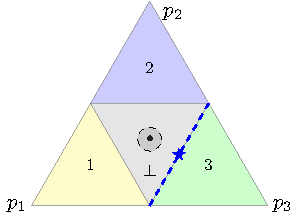
\includegraphics[width=\linewidth]{tikz/fsd-bound.pdf}
%	\caption{%Since the uniform distribution is in the relative interior of the simplex and the level set $\gamma_\bot$, 
%          $\dim(\Sc_{\gamma_\bot}($\textbullet$)) = 2$ and $\dim(\Sc_{\gamma_\bot}({\color{blue}\star})) = 1$.}
%	\label{fig:fsd-bound}
%\end{minipage}
%\hfill
%\begin{minipage}{0.45\linewidth}
%	\centering
%	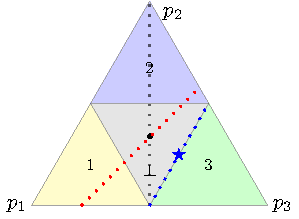
\includegraphics[width=\linewidth]{tikz/flats-bound.pdf}
%	\caption{Any $1$-flat $F$ through \textbullet leaves $\gamma_\bot$.
%	However, there is a $1$-flat containing ${\color{blue}\star}$ that is a subset of $\gamma_\bot$ and $\gamma_3$.
%	}
%	\label{fig:flats-bound}
%\end{minipage}
%\end{figure}


\begin{figure}[htb]
	\centering
	\begin{tabular}{cc}
%				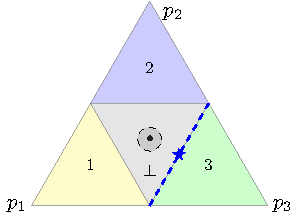
\includegraphics[width=.35\textwidth]{tikz/fsd-bound.pdf} & 
%				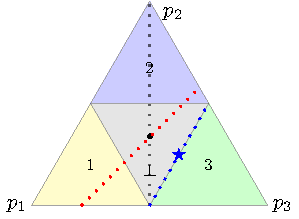
\includegraphics[width=.35\textwidth]{tikz/flats-bound.pdf} \\
	\end{tabular}
	\caption{(Left) Feasible subspace dimension $\Sc_{\gamma_\bot}(\bullet) = 2$ and $\Sc_{\gamma_\bot}({\color{blue}\star}) = 1$, giving the bound $\conscvx(\ell^{abs}) \geq 3- 1-1 = 1$.
		(Right) No $1$-flat through $\bullet$ (a line since $\bullet \in \relint{\simplex})$  stays fully contained in $\gamma_\bot$, so $\conscvx(\ell^{abs}) \geq 2$.\jessie{FIX FIGURES}}
	\label{fig:fsd-flats-abstain}
\end{figure}


\section{Reconstructing \citet[Thm.\ 16]{ramaswamy2016convex}}



\begin{lemma}\label{lem:finite-relint-dim}
  Let the $d$-flat $F\subseteq \P$ (defined over finite $\Y$) contain some $p\in\relint{\P}$.
  Then 
  \begin{enumerate}
  	\item[(i)] $p \in \relint{F}$; 
  	\item[(ii)] $\dim(\Scr_F(p)) \geq \dim(\affhull(\P)) - d$.
  \end{enumerate}
\end{lemma}
%\jessiet{Bo had a good point that $\spn(F_p)$ is probably easier to understand, instead of having an extra layer of notation in there.  Do we want to stick with $\Scr_F(p)$ or $\spn(F_p)$?}
%\raft{True, but the reader doesn't know $F_p$ anymore, since it's within the proof.  Plus, this is the statement we really need.  So I'd vote sticking with $\Scr_F$.}
\begin{proof}
  %\raf{Moved; see margin comment:  for the function $W : \Y \to \reals^d$ such that $F = \zeros{W}$.  (Such a function must exist by $F$ being a $d$-flat.)}
  
  As $F$ is a $d$-flat, we have some $W:\Y \to \reals^d$ such that $F = \zeros{W}$.
  Throughout, given a point (typically a distribution) $p$ and convex set $P$, we define $P_p := P - \{p\}$.
  Define $T_W:\spn(\P_p)\to\reals^d, v\mapsto \E_v W$.
  
  (i)
  Since $p \in \relint{\P}$, for all $q \in \P$, there is some small enough $\epsilon > 0 $ so that for all $\alpha \in (-\epsilon,\epsilon)$, the point $q_\alpha := p - \alpha(q - p)$ is still in $\P$.
  In particular, for $q \in F$, we claim $q_\alpha \in F$.
  %\raft{$V$ comes out of nowhere here, and then in the next bullet you introduce $W$ for the same thing. Better to do all that before both bullets. ``As $F$ is a $d$-flat, we have some $W$... $F=\zeros{W}$''.  Also, okay to just write $\E_p W$ not $\E_p W(Y)$, since technically $W$ is a random variable.}
  As $p,q \in F$, we have $\E_pW = \E_qW = \vec 0$.
  By linearity of expectation, we then have $\E_{q_\alpha} W = \vec 0$.
  % (Y) = \E_p V(Y) - \alpha(\E_q V(Y) - \E_p V(Y)) = \vec 0 - \alpha(\vec 0 - \vec 0) = \vec 0$.
  This implies $q_\alpha \in F$, and therefore $p \in \relint{F}$.
  
  (ii)
  We first show $\spn(F_p) = \Scr_F(p)$.
  First, take $v \in \Scr_F(p)$, and take $\epsilon_0$ as in the definition.
  For $\epsilon = \epsilon_0 / 2$, we then have $p + \epsilon v \in F \implies \epsilon v \in F_p$, and therefore, $v \in \spn(F_p)$.  
  Now take $v \in \spn(F_p)$.
  Since $p \in \relint{F}$ (i), we have $\vec 0 \in \relint{F_p}$.
  Therefore there is an $\epsilon_0 > 0$ so that $\epsilon v \in F_p$ for all $\epsilon \in (-\epsilon_0, \epsilon_0)$ by convexity of $F$.
  Therefore, $v \in \Scr_F(p)$, and we observe $\Scr_F(p) = \spn(F_p)$.
  
  We now show $\Scr_F(p) = \ker(T_W)$.
%  Let $v \in \ker(T_W)$. % = \{v \in \spn(\P_p) : T_W(v) = \vec 0\}$.
%  From (i), as $p \in \relint{\P}$, we have $\vec 0 \in \relint{F_p}$.
%  Thus there is some $\epsilon > 0$ so that $\epsilon v \in F_p$ and $-\epsilon v \in F_p$.
%  As $\epsilon v \in F_p$, and $v$ is a scalar multiple of it, we additionally conclude $v \in \spn(F_p)$.
%  Moreover, we have $\pm \epsilon v \in \ker(T_W)$ by linearity of expectation, so $v \in \relint{\ker(T_W)}$.
%  Hence, $\spn(F_p) = \ker(T_W)$.\jessie{Right?}\raf{Why? Hint: you want to show $v$ is in the span of $F_p$; in fact, it's a scalar multiple of something in $F_p$.}
%  
%  more up to date than above; commented out 1.25.21
%  Let $v \in \Scr_F(p)$.
%  Then there is some $\alpha$ so that $\alpha v \in F_p$.
%  This means $\E_{\alpha v} W = \vec 0$, which in turn implies $\alpha v \in \ker(T_W)$.
%  By linearity of expectation, we additionally have $v \in \ker(T_W)$.
%  Thus, $\Scr_F(p) \subseteq \ker(T_W)$.
%
  Observe that $\Scr_F(p) \subseteq \ker(T_W)$ follows trivially from the definitions of the two functions. 
  Now let $v \in \ker(T_W)$, and $v' \in F_p$.
  This means $\E_v W = \vec 0$, so it suffices to show $v = c v' \in F_p$, thus showing $v \in \Scr_F(p)$.
  Since $p \in \relint{\P}$, we must have $\vec 0 \in \relint{F_p}$, so we know there is some small enough $\epsilon > 0$ so that $-\alpha v' \in F_p$ for $\alpha \in (-\epsilon, \epsilon)$.
  Take $c = -\alpha$, and we conclude $v \in \Scr_F(p)$.
  Therefore, $\ker(T_W) = \Scr_F(p)$.

  \jessiet{Check me; this is hand wavy, but I'm okay with it or submission!}  
  We finally want to show $\dim(\affhull(\P)) = \dim(\spn(\P_p))$.
  Consider that any $q \in \spn(\P_p)$ can be written as a scalar multiple of an element of $\P_p$, which can be written as a convex combination of elements of the minimal basis $\P_p$.
  In particular, since $\vec 0 \in \P_p$, it can be written as an affine combination of elements of the basis, so $\dim(\affhull(\P)) \geq \dim(\spn(\P_p))$.
  We also have $\affhull(\P) - \{p\} \subseteq \spn(\P_p)$, so $\dim(\affhull(\P)) = \dim(\affhull(\P) - \{p\}) \leq \spn(\P_p)$.
  Therefore, $\dim(\affhull(\P)) = \dim(\spn(\P_p))$.

  
  As $\Y$ is a finite set, $\spn(\P_p)$ is a finite-dimensional vector space.
  The rank-nullity theorem states $\dim(\im(T_W)) + \dim(\ker(T_W)) = \dim(\spn(\P_p)) = \dim(\affhull(\P))$.
  As $\dim(\im(T_W)) \leq d$, and we have shown above that $\Scr_F(p) = \spn(F_p) = \ker(T_W)$, the conclusion follows.
  % 
  %	Now let $v \in \ker(T_W) = \{v \in \spn(\P_p) : T_W(v) = \vec 0\}$.
  %	There must exist an $\epsilon > 0$ so that $\epsilon v \in F_p$ and $-\epsilon v \in F_p$ $p \in \relint{\P}$ implies $\vec 0 \in \relint{F_p}$ by (1.).
  %	Moreover, we have $\pm \epsilon v \in \ker(T_W)$ by linearity of expectation, so $v \in \relint{\ker(T_W)}$.
  %	This allows us to conclude $\spn(F_p) = \ker(T_W)$.\jessie{Right?}
  %	
  %	We want to show $F_p = \P_p \cap \ker(T_W)$, then derive the result from there. \jessie{I don't see why this is necessary.}
  %	
  %	In order to see this, consider $v \in F_p \iff v + p \in F$, and similarly for $\P_p$.
  %	Now, as $F \subseteq \P$ by construction, we have $F_p \subseteq \P_p$, and since $\spn(F_p) = \ker(T_W)$, we additionally have $F_p \subseteq \ker(T_W)$, yielding $F_p \subseteq \P_p \cap \ker(T_W)$.
  %	Now consider $v \in \P_p \cap \ker(T_W)$; we know that $\E_v W = \vec 0$, and therefore, $\E_{q} W = \vec 0$, so $v \in F_p$, thus $F_p = \P_p \cap \ker(T_W)$.
  %	
  %	Since $\spn(F_p) = \ker(T_W)$, we have $\dim(\spn(F_p)) = \dim(\ker(T_W)) \geq \dim(\spn(\P_p)) - d$ by \jessie{isomorphism theorem} since $F_p = \ker(T_W) \cap \P_p$. \jessie{??}
\end{proof}

% Commented out 01.26.2021 - Jessie to simplify proof of \hariresult
%\begin{lemma}\label{lem:Fp-subset-feasible-subset}
%Suppose we are given $p \in \relint{\P}$, property $\gamma: \P \toto \R$, and report $r \in \gamma(p)$.
%If $\gamma$ is indirectly elicited by a convex $L \in \L_d$, then there is a $d$-flat $F$ such that $p \in F$ and $F_p \subseteq \Sc_{\gamma_r}(p)$.	
%\end{lemma}
%\begin{proof}
%	Construct $F$ as in Lemma~\ref{lem:convex-flats-inf-dim}; $F$ is a $d$-flat, contains $p$, and we have $F \subseteq \gamma_r$.
%	We aim to show $v \in F_p \implies v \in \Sc_{\gamma_r}(p)$.
%	By Lemma~\ref{lem:finite-relint-dim}(i), we know $p \in \relint{F}$, and therefore, $\vec 0 \in \relint{F_p}$.
%	Consider $v \in F_p$.
%	By $F_p$ being convex and $\vec 0 \in \relint{F_p}$, we know there exists an $\alpha > 0$ so that $-\alpha v \in F_p$.
%	This implies $p - \alpha v \in F \implies p - \alpha v \in \gamma_r \implies v \in \Sc_{\gamma_r}(p)$ since $F$ and $\Sc_{\gamma_r}(p)$ are convex and $F \subseteq \gamma_r$.
%	This yields the desired result, $F_p \subseteq \Sc_{\gamma_r}(p)$.\raft{It feels weird how redundant this is from the argument in the 1st paragraph of (ii) above, but okay for now.}
%\end{proof}



%\begin{lemma}\label{lem:feas-sub-is-a-flat}
%	Suppose we have the discrete elicitable property $\gamma$ and distribution $p \in \relint{\simplex}$ with $r \in \gamma(p)$.
%	If $F$ is a flat so that $p \in F \subseteq \gamma_r$, then $F' := F - \{p\}$ is contained in $\Sc_{\gamma_r}(p)$.
%	%  \raf{I think you want $p$ in the interior of the simplex for now}
%\end{lemma}
%\begin{proof} \jessie{Better to combine; not currently using this}
%	We aim to show $v \in F' \implies v \in \Sc_{\gamma_r}(p)$.
%	First, observe $v \in F' \iff p + v \in F$.
%	As $p \in \relint{\simplex}$, by Lemma~\ref{lem:finite-relint-dim}, we additionally have $p \in \relint{F}$, and in turn $\vec 0 \in \relint{F'}$.
%	
%	Suppose $v \in F'$, and since $p \in \relint{F}$, there is an $\epsilon > 0$ so that for all $\alpha \in (-\epsilon, \epsilon)$, we have $p + \alpha v \in F \implies p + \alpha v \in \gamma_r$, since $F$ is convex.%, as are level sets of elicitable properties~\cite{lambert2009eliciting}.
%	The result follows by applying the definition of Feasible Subspaces.
%	%By definition of $\Sc_{\gamma_r}(p)$, there is then an $\epsilon$ satisfying the requirement for $v \in \Sc_{\gamma_r}(p)$, so we can conclude $v \in \Sc_{\gamma_r}(p)$, yielding the desired result.
%	
%% %commented out 01.21.2021 - Jessie
%%	\jessie{Revisit this proof}
%%	Observe $F-p$ is a subspace as it is a linear shift of $F$, which is a linear subspace by definition of a flat and the fact that it contains $\vec 0$ (since $F$ contains $p$, which we subtract from).
%%	Now consider $v \in F - p$.
%%	Since $p \in \relint{\P}$, there is an open ball of radius $\epsilon$ in the span of $\P$ so that for all $q \in B(p, \epsilon)$, we have $q \in \P$.
%%	In particular, take $\alpha = \epsilon / 2$, and we observe $p \pm \alpha v \in B(p, \epsilon)$, and therefore $p \pm \alpha v \in \P$.
%%	Moreover, by the assumption $v \in F - p$, we also have $p \pm \alpha v \in \gamma_r$. 
%%	Since level sets of elicitable properties are convex (\citep{lambert2009eliciting}) this is true for all $\alpha' \in [0,\alpha]$.
%%	Therefore, we observe $v \in S_{\gamma_r}(p)$, so $F-p \subseteq S_{\gamma_r}(p)$.
%\end{proof}


\newcommand{\simplexp}{\Delta_{\Y'}}

%commenting out 01.25.2021 since we really just need one direction.
%\begin{lemma}\label{lem:p-boundary-fsd}
%	For any $p \in \P$ and $r$ such that $p \in \gamma_r$, take $\Y' := \supp(p)$.
%	Define $\gamma' : \P \toto \R$ with $\gamma' : q \mapsto \gamma(q) \cap \simplexp$.
%	Then $\Sc_{\gamma_r}(p) = \Sc_{\gamma'_r}(p)$.
%\end{lemma}
%\begin{proof}
%	Consider the ambient space of both $\Sc_{\gamma_r}(p)$ and $\Sc_{\gamma'_r}(p)$ is $\reals^\Y$.
%	We trivially have $\dim(\Sc_{\gamma_r}(p)) \geq \dim(\Sc_{\gamma'_r}(p))$ since $\gamma'$ is simply $\gamma$ projected down to an affine subspace of $\reals^\Y$.
%	
%	Now to see $\dim(\Sc_{\gamma_r}(p)) \leq \dim(\Sc_{\gamma'_r}(p))$, it suffices to show subset inclusion.
%	Take some $v \not \in \Sc_{\gamma'_r}(p)$.
%	Observe that $\gamma'_r = \gamma_r \cap \simplexp$, so if $q^\pm := p \pm \epsilon v \not \in \gamma'_r$ for all $\epsilon > 0$ (i.e. $p \not \in \relint{\simplexp}$), it is either because one of $q^+$ or $q^-$ is not in $\gamma_r$ or because either $q^\pm \not \in \simplexp$.
%	The first case can be seen easily by the definition of $\gamma'$, and the latter can be seen because leaving $\simplexp$ means one of $q^\pm$ also is not in $\P$, and therefore not in $\gamma_r$ as $\gamma_r \subseteq \P$.
%	Thus $\Sc_{\gamma_r}(p) = \Sc_{\gamma'_r}(p)$.
%	%commented out 05.26.2020
%	%	For simplicity, consider $\epsilon = \epsilon_0 / 2$.
%	%	Consider $P := \spn(\{e_y : y \in \supp(p) \})$.
%	%	\begin{align*}
%	%	\dim(\Sc'_{\gamma_r}(p)) &= \dim(\Sc_{\gamma_r}(p)) + \dim(P) - \dim(\Sc_{\gamma_r}(p) + P)
%	%	\end{align*}
%	%	If $\dim(P) = \dim(\Sc_{\gamma_r}(p) + P)$, the claim holds.
%	%	Be definition of $P$, we know $\dim(P) = \|p\|_0$, so we can show $\dim(\Sc_{\gamma_r}(p) + P) = \|p\|_0$.		
%	%	One way to do this is to show $\Sc_{\gamma_r}(p) \subseteq P$.
%	%	
%	%	Suppose there was some $v \not\in P$ such that $v \in \Sc_{\gamma_r}(p)$.
%	%	That means there is some $i$ so that $i \not \in \supp(p)$ (i.e. $p_i = 0$) but $v_i \neq 0$. \jessiet{Check this line.}
%	%	However, if $v \in \Sc_{\gamma_r}(p)$, then there is some $\epsilon_0 > 0$ so that $p + \epsilon v$ and $p - \epsilon v \in \gamma_r \subseteq \simplex$ for all $\epsilon \in (0, \epsilon_0)$.
%	%	For simplicity, consider $\epsilon = \epsilon_0 / 2$.
%	%	Since $p_i = 0$, this gives $(p+\epsilon v)_i = (\epsilon v)_i$, and likewise for $(p - \epsilon v)_i$.
%	%	As neither $\epsilon$ nor $v_i$ are $0$, one of these terms must be negative, and therefore not in the simplex.
%	%	As $\gamma_r \subseteq \simplex$, we then have $v \not \in \Sc_{\gamma_r}(p)$.
%	%	Therefore, $\Sc_{\gamma_r}(p) \subseteq P$, and $\dim(\Sc_{\gamma_r}(p) + P) = \dim(P) = \|p\|_0$.
%\end{proof}

\hariresult*
\begin{proof}
  Let $L \in \Lcvx_d$ be a calibrated surrogate for $\ell$, and let $\Gamma := \prop[\simplex]{L}$.
  Consider $\Y' := \{y\in\Y : p_y > 0\}$ and $p' = (p_y)_{y\in\Y'} \in \Delta_{\Y'}$.
  Take $L' := L|_{\Y'}$ and $\ell' := \ell|_{\Y'}$.
  Define $h:\reals^{\Y'} \to \reals_\Y$ such that $h(q') = q$ such that $q_y = q'_y$ for $y\in\Y'$ and $q_y = 0$ otherwise.
  Take $\Gamma' = \Gamma \circ h$, $\gamma' = \gamma \circ h$.
  
  \raf{Show that $L'$ indirectly elicits $\gamma'$.}
  We wish to first  show $L'$ indirectly elicits $\gamma'$.
  Since $L$ indirectly elicits $\gamma$, we have a link $\psi$ such that for all $u \in \reals^d$, $\Gamma_u \subseteq \gamma_{\psi(u)}$.
  As $\Gamma'(q) = \Gamma(h(q))$ and $\gamma'(q) = \gamma(h(q))$\jessiet{Hand waving}, we have $q \in \Gamma'_u \iff h(q) \in \Gamma_u \implies h(q) \in \gamma_{\psi(u)} \iff (q_y)_{y \in \Y'} \in \gamma'_{\psi(u)}$, and therefore, $L'$ indirectly elicits $\gamma'$ via the link $\psi \circ \proj(\Y')$, where $\proj(\Y') : q \mapsto (q_y)_{y \in \Y'}$. 
%  By consistency, we have $L$ indirectly eliciting $\gamma$.
%  Now, observe $L'$ (eliciting $\Gamma'$) indirectly elicits $\gamma' := \prop[\simplexp]{\ell'}$ since, for all $q \in \simplex$, taking $B : q \mapsto \{q_{y} \mid y > 0\}$, and in particular, $p' = B(p)$, we have $p' \in \Gamma'_u \implies p' \in \gamma'_{\psi(u)}$.
%  Moreover, $\Gamma(p) = \Gamma'(p')$ and $\gamma(p) = \gamma'(p')$.
%  This same observation can be used to observe that $L'$ is also calibrated with respect to $\ell'$ as the calibration bound holds for all $q \in \simplex$, and .

  \raf{Show $\dim(\Sc_{\gamma_r}(p)) \geq \dim(\Sc_{\gamma'_r}(p'))$}
\jessie{  Let $\{v_i\}_{i=1}^k$ form a basis for $\Sc_{\gamma_r}(p)$.
  If there is some $v' \in \Sc_{\gamma'_r}(p')$ that cannot be written as $\sum_{i=1}^k \alpha_i v_i$, then we claim $\{v_i\}_{i=1}^k$ does not form a basis for $\Sc_{\gamma_r}(p)$.
  In particular, consider $q := h(v' + p')$; we have $q \in \gamma_r$ since $v' + p' \in \gamma'_r$, and $q - p \in \Sc_{\gamma_r}(p)$ via the same $\epsilon_0$ that allows $v' \in \Sc_{\gamma'_r}(p')$.
  However, as $v'$ cannot be written $\sum_{i=1}^k \alpha_i v_i$, neither can $v' + p'$.
  As $h$, by construction, does not change the dimension of its argument, we have $q$ cannot be written as $\sum_{i=1}^k \alpha_i v_i$, so we have $\{v_i\}_{i=1}^k$ is not a basis for $\Sc_{\gamma_r}(p)$.
  Thus, we have $\dim(\Sc_{\gamma_r}(p)) \geq \dim(\Sc_{\gamma'_r}(p'))$.}
  
We aim to show $\dim(\Sc_{\gamma_r}(p)) \geq \dim(\Sc_{\gamma'_r}(p'))$.
  We do this by showing that $h(\Sc_{\gamma'_r}(p')) \subseteq \Sc_{\gamma_r}(p)$, and the result holds as $h$ is linear and injective.
Suppose $v \in h(\Sc_{\gamma'_r}(p'))$, then there exists a $v'$ so that $v = h(v')$ and an $\epsilon_0 > 0$ such that $\epsilon v' + p' \in \gamma'_r$ for all $\epsilon \in (-\epsilon_0, \epsilon_0)$.
Since $h$ is linear and recall $h(\gamma'_r) \subseteq \gamma_r$, this implies $\epsilon v + p \in \gamma_r$ for all $\epsilon \in (-\epsilon_0, \epsilon_0)$.
Therefore $v \in \Sc_{\gamma_r}(p)$, and the result follows. 
  
%  Consider $\gamma_r = h(\gamma'_r) = \{h(q') \mid q' \in \gamma'_r\}$.
%  Then $v \in \Sc_{\gamma_r}(h(p')) \implies \exists \epsilon_0$ so that $h(p') + \epsilon v \in \gamma_r \forall \epsilon \in (-\epsilon_0, \epsilon_0)$ if and only if $p' + \epsilon v \in \gamma'_r \forall \epsilon \in (-\epsilon_0, \epsilon_0)$.
%  Moreover, we have $\Sc_{\gamma_r}(p) \supseteq \Sc_{\gamma'_r}(p')$...
  
  As $L'$ indirectly elicits $\gamma'$, by Corollary~\ref{cor:Pcodim-flat-elic-relint-prop}, we know there exists a $d$-flat $F$ with $p' \in F \subseteq \gamma'_r$.
  Taking $\P = \simplexp$, we know $p' \in \relint{\simplexp}$ by construction, so we can apply Lemma~\ref{lem:finite-relint-dim}(ii), which gives $\dim(\Scr_F(p')) \geq  \dim(\affhull(\simplexp)) - d = \|p\|_0 - 1-d$.\footnote{To reason about $\dim(\affhull(\simplexp)) = \|p\|_0 - 1$, observe that the uniform distribution on $\simplexp$ has full support and therefore requires $\|p\|_0 - 1$ elements in its basis.}
  % which gives $\dim(\Scr_F(p')) \geq \dim(\spn(\P_{p'})) - d$.
  % Since $\P = \simplexp$ and $p' \in \relint{\simplexp}$, we have $\dim(\spn(\P_{p'})) = \dim(\affhull(\simplexp)) = \|p\|_0 - 1$. \jessie{How to get rid of sub p notation here?}
  % Therefore, $\dim(\spn(F_p)) \geq \|p\|_0 - 1 - d$
  \raft{Might be nicer on the reader to add one more step for $\|p\|_0$. Also, I just realized we are using $p\in\simplex$ here, but then $p$ can't be in $F\subseteq\Delta_{\Y'}$ ($p$ is an $n$-vector). So maybe we need a $p'$ too.\jessie{Is this better now?  Slash can we remove this comment?}}
  Additionally, $\Scr_F(p') \subseteq \Sc_{\gamma'_r}(p')$ by subset inclusion of the sets themselves.
  % By Lemma~\ref{lem:p-boundary-fsd}, we additionally have $\Sc_{\gamma_r}(p) = \Sc_{\gamma'_r}(p')$.
  Chaining these results, we obtain 
  \begin{align*}
    \dim(\Sc_{\gamma_r}(p)) &\geq \dim(\Sc_{\gamma'_r}(p'))  \geq \dim(\Scr_F(p')) \geq \|p\|_0 - 1 - d~.~
  \end{align*}
  % 
  %	this yields the bound $\dim(\spn(F-\{p\})) \geq \|p\|_0 - 1 - d$.
  %	Chaining inequalities, we then have $\dim(\Sc_{\gamma'_r}(p)) \geq \dim(\spn(F - \{p\})) \geq \|p\|_0 - d- 1$ as Lemma~\ref{lem:feas-sub-is-a-flat} states $F - \{p\}$ is a subspace of $\Sc_{\gamma'_r}(p)$.
  %	Lemma~\ref{lem:p-boundary-fsd} then states $\dim(\Sc_{\gamma'_r}(p)) = \dim(\Sc_{\gamma_r}(p))$, and from there we observe the result.
  % 
  % 
  % \old version of the proof from NeurIPS or before - 01.21.2021
  %	First, for intuition, consider $p \in \relint{\simplex}$. 
  %	Theorem~\ref{thm:cvx-flats} implies that there exists a flat $F'$ of affine dimension at least $n-d-1$.
  %	Lemma~\ref{lem:feas-sub-is-a-flat} then says that $\dim(\Sc_{\gamma_r}(p)) \geq \dim(F') \geq n-d-1 \implies d \geq n - \dim(\Sc_{\gamma_r}(p)) - 1$.
  % 
  %	
  %	If we can show that $L' := L|_{\Y'}$ is calibrated with respect to $\ell' := \R \times \Y' \to \reals$ with $\ell(r,y) = \ell'(r,y)$ for all $r \in \R$ and $y \in \Y'$ and indirectly elicits $\gamma' := \prop{\ell'}$, then we observe the existence of a flat $F^*$ of codimension $d$ (in $\reals^{\Y'}$) so that $\dim(F^*) = \|p\|_0 - d - 1$ by Theorem~\ref{thm:cvx-flats}.
  %	Then we can use Lemma~\ref{lem:p-boundary-fsd} to observe $\dim(\Sc_{\gamma'_r}(p)) = \dim(\Sc_{\gamma_r}(p))$, and thus the result holds.
  %	
  %	Now to see that $L'$ is calibrated with respect to $\ell'$, consider that $\gamma(p) = \gamma'(p)$ for all $p \in \Delta^{\Y'}$,
  %	\begin{align*}
  % \forall p \in \Delta_{\Y'}:  \inf_{u \in \reals^d : \psi(u) \not \in \gamma'(p)} L'(u;p) = \inf_{u \in \reals^d : \psi(u) \not \in \gamma(p)} L(u;p) > \inf_{u \in \reals^d} L(u;p) = \inf_{u \in \reals^d} L'(u;p)~.~
  % \end{align*}
  %	Therefore, we have $L'$ calibrated with respect to $\ell'$.
  % 
  %	Moreover, we want to show $L'$ indirectly elicits $\gamma'$ so we can apply Theorem~\ref{thm:cvx-flats}.
  %	First, observe that $L'$ elicits $\Gamma' : p \mapsto \Gamma(p)$ for all $p \in \Delta_{\Y'}$ 
  %	For all $p \in \simplex$, we have $u \in \Gamma(p) \implies \psi(u) \in \gamma(p)$.
  %	As $\Delta_{\Y'} \subseteq \simplex$, this is in particular true for all $p \in \Delta_{\Y'}$.
  %	Therefore, for all $p \in \Delta_{\Y'}$, we have $\Gamma'_u = \Gamma_u \cap \Delta_{\Y'} \subseteq \gamma_{\psi(u)} \cap \Delta_{\Y'} = \gamma'_{\psi(u)}$, and thus $L'$ indirectly elicits $\gamma'$.
\end{proof}

\section{Proof of Theorem~\ref{thm:bayes-risk-lower-bound}}\label{app:pf-bayesrisklowerbound}

\newcommand{\EL}{\mathcal{E}}
\newcommand{\defeq}{:=}
\newcommand{\conv}{\mathrm{conv}}

\subsection{General setting of elicitation complexity}

We briefly introduce the general notion of elicitation complexity, of which Definition~\ref{def:cvx-elic-complex} is a special case, as some statements are more naturally made in this general setting.

\begin{definition}
  \label{def:refine}
  $\Gamma'$ \emph{refines} $\Gamma$ if for all $r'\in\range\Gamma'$ there exists $r\in\range\Gamma$ with $\Gamma'_{r'} \subseteq \Gamma_r$.
\end{definition}
Equivalently, $\Gamma'$ refines $\Gamma$ if there is a link function $\psi:\range\Gamma'\to\range\Gamma$ such that $\Gamma'_{r'} \subseteq \Gamma_{\psi(r')}$ for all $r'\in\range\Gamma'$.

\begin{definition}
  \label{def:el}
  For $k\in\mathbb{N}\cup\{\infty\}$, let $\EL_k(\P)$ denote the class of all elicitable properties $\Gamma:\P\to\reals^k$, and $\EL(\P) \defeq \bigcup_{k\in\mathbb{N}\cup\{\infty\}} \EL_k(\P)$.
  When $\P$ is implicit we simply write $\EL$.
\end{definition}

\begin{definition}
  \label{def:elic-complex}
  Let $\C$ be a class of properties.
  % A property $\Gamma$ is \emph{$k$-elicitable with respect to $\C$}
  % if there exists an intermediate property  and which refines $\Gamma$.
  The \emph{elicitation complexity} of a property $\Gamma$ with respect to $\C$, denoted  $\elic_\C(\Gamma)$, is the minimum value of $k\in\mathbb{N}\cup\{\infty\}$ such that there exists $\hat \Gamma \in \C\cap\EL_k(\P)$ that refines $\Gamma$.
\end{definition}


\subsection{Supporting statements}

\begin{proposition}[\citet{osband1985providing}]
  \label{prop:elic-complex-level-sets-convex}
  Let $\Gamma$ be elicitable.
  Then $\Gamma_r$ is convex for all $r\in\range\Gamma$.
\end{proposition}

\begin{lemma}[{Set-valued extension of \citet[Lemma 4]{frongillo2020elicitation}}]
  \label{lem:refine}
  If $\Gamma'$ refines $\Gamma$ then $\elic_\C(\Gamma') \geq \elic_\C(\Gamma)$.
\end{lemma}

\begin{proof}
  As $\Gamma'$ refines $\Gamma$, we have some $\psi:\range\Gamma'\to\range\Gamma$ such that for all $r'\in \range\Gamma'$ we have $\Gamma'_{r'} \subseteq \Gamma_{\psi(r')}$.
  Suppose we have $\hat\Gamma\in\C$ and $\varphi:\range\hat\Gamma\to\range\Gamma'$ such that for all $u\in \range\hat\Gamma$ we have $\hat\Gamma_u \subseteq \Gamma'_{\varphi(u)}$.
  Then for all $u\in \range\hat\Gamma$ we have $\hat\Gamma_u \subseteq \Gamma'_{\varphi(u)} \subseteq \Gamma_{(\psi \circ \varphi)(u)}$.
  In particular, if $\elic_\C(\Gamma') = m$, then we have such a $\hat\Gamma:\P\toto \reals^m$, and hence $\elic_\C(\Gamma) \leq m$.
  \raft{The logic for this whole proof could use a very careful check}
\end{proof}

\begin{lemma}[{\citet[Lemma 8]{frongillo2020elicitation}}]
  \label{lem:elic-complex-bayes-concave}
  Suppose $L \in \L$ elicits $\Gamma:\P\to\R$ and has Bayes risk $\lbar$.
  Then for any $p,p'\in\P$ with $\Gamma(p)\neq\Gamma(p')$, we have $\lbar(\lambda p + (1-\lambda) p') > \lambda \lbar(p) + (1-\lambda) \lbar(p')$ for all $\lambda\in(0,1)$.
\end{lemma}

\begin{lemma}[{Adapted from \citet[Theorem 4]{frongillo2020elicitation}}]
  \label{lem:bayes-risk-lower-bound}
  If $L$ elicits a single-valued $\Gamma$, and $\hat\Gamma$ refines $\lbar$, then $\hat\Gamma$ refines $\Gamma$.
\end{lemma}
\begin{proof}
  Suppose for a contradiction that $\hat\Gamma$ does not refine $\Gamma$.
  Then we have some $u\in\range\hat\Gamma$ such that for all $r\in\range\Gamma$ we have $\hat\Gamma_u \not\subseteq \Gamma_r$.
  In particular, recalling that $\Gamma$ is single-valued, we must have $p,p'\in\hat\Gamma_u$ such that $\Gamma(p) \neq \Gamma(p')$.
  Moreover, as $\hat\Gamma$ refines $\lbar$, we also have $\lbar(p) = \lbar(p')$.
  From Lemma~\ref{lem:elic-complex-bayes-concave} and $\lambda=1/2$ we have $\lbar(q) > \tfrac 1 2 \lbar(p) + \tfrac 1 2 \lbar(p') = \lbar(p)$, where $q = \tfrac 1 2 p + \tfrac 1 2 p'$.
  As the level set $\hat\Gamma_u$ is convex by Proposition~\ref{prop:elic-complex-level-sets-convex}, we also have $q \in \hat\Gamma_u$, and hence $\lbar(q)=\lbar(p)$, a contradiction.
\end{proof}

\begin{lemma}[Minor modifications from \citet{frongillo2020elicitation}]\label{lem:lin-alg-nested-level-sets}
  Let $\V$ be a real vector space.
  Let $f:\V\to\reals^k$ be linear and $C\subseteq \V$ convex with $\spn C = \V$, and let $m\in\mathbb{N}$.
  Suppose that $0 \in \interior f(C)$, and
  for all $v\in S \defeq C \cap \ker f$, there exists a linear $\hat f_v:\V\to\reals^m$ with $v \in C \cap \ker \hat f_v \subseteq S$.
  Then $m \geq k$.
  If $m=k$, we additionally have $0\in\interior\hat f_v(C)$ for some $v\in S$.
  \raft{I changed the statement to reflect the proof better, but did not change the proof apart from $\hat f \to \hat f_v$.  Could still use a careful check though!}
\end{lemma}
\begin{proof}
  The condition $0 \in \interior f(C)$ is equivalent to the existence of some $v_1,\ldots v_{k+1} \in C$ such that $0\in\interior\conv\{f(v_i) : i\in\{1,\ldots,k+1\}\}$.
  Let $\alpha_1,\ldots,\alpha_{k+1}>0$, $\sum_{i=1}^{k+1} \alpha_i = 1$, such that $\sum_{i=1}^{k+1} \alpha_i f(v_i) = 0$.
  As these are barycentric coordinates,
  this choice of $\alpha_i$ is unique, a fact which will be important later.
  We will take $v = \sum_{i=1}^{k+1} \alpha_i v_i$, an element of $C$ by convexity, and thus an element of $S$ as $f(v)=0$.

  Let $\hat f_v:\V\to\reals^m$ be linear with $v \in \hat S := C \cap \ker \hat f_v \subseteq S$.
  Let $\beta_1,\ldots,\beta_{k+1}\in\reals$, $\sum_{i=1}^{k+1} \beta_i = 0$, such that $\sum_{i=1}^{k+1} \beta_i \hat f_v(v_i) = 0$.
  We will show that the $\beta_i$ must be identically zero, i.e. that $\{\hat f_v(v_i):i\in\{1,\ldots,k+1\}\}$ are affinely independent.
%  \raft{We want to show that the $\beta_i$ must be 0 (that's one definition of affine independence)}
  By construction, $v' := \sum_{i=1}^{k+1} \beta_iv_i \in \ker \hat f_v$, and as $v\in\ker\hat f_v$, for all $\lambda > 0$ we have $v_\lambda := v + \lambda v' = \sum_{i=1}^{k+1} (\alpha_i + \lambda \beta_i) v_i \in \ker \hat f_v$.
  Taking $\lambda$ sufficiently small, we have $\gamma_i := \alpha_i + \lambda \beta_i > 0$ for all $i$, and $\sum_{i=1}^{k+1} \gamma_i = \sum_{i=1}^{k+1} \alpha_i + \lambda\sum_{i=1}^{k+1} \beta_i = 1$.
  By convexity of $C$, we have $v_\lambda \in C$.
  Now $v_\lambda \in C \cap \ker \hat f_v \subseteq S = C \cap \ker f$, and in particular $v_\lambda \in \ker f$.
  Thus, $f(v_\lambda) = \sum_{i=1}^{k+1} \gamma_i f(v_i) = 0$.
  By the uniqueness of barycentric coordinates, for all $i\in\{1,\ldots,k+1\}$, we must have $\gamma_i = \alpha_i$ and thus $\beta_i = 0$, as desired.

  As $\hat f_v(C)$ contains $k+1$ affinely independent points, we have $m \geq \dim \im \hat f_v \geq k$.
  When $m=k$,
  by affine independence, the set $\conv\{\hat f_v(v_i) : i\in\{1,\ldots,k+1\}\}$ has dimension $k$ in $\reals^k$.
  As $0 = \hat f_v(v) = \sum_{i=1}^{k+1} \alpha_i \hat f_v(v_i)$, and $\alpha_i > 0$ for all $i$, we conclude $0\in\interior\conv\{\hat f_v(v_i) : i\in\{1,\ldots,k+1\}\} \subseteq \interior \hat f_v(C)$.
\end{proof}

\begin{lemma}[{\citet[Lemma 14]{frongillo2020elicitation}}]
  \label{lem:lin-alg-span}
  Let $\V$ be a real vector space.
  Let $f:\V\to\reals^k$ be linear, $C\subseteq \V$ convex with $\spn C = \V$, and let $S = C \cap \ker f$.
  If $0 \in \interior f(C)$ then $\spn S = \ker f$.
\end{lemma}

\subsection{Proving the lower bound for spectral risks \raf{Bayes risks, not spectral!}}

Let $\C^*_d$ be the class of properties $\Gamma$ which are elicited by a convex loss $L\in\Lcvx_d$ for some $d\in\mathbb{N}$, and let $\C^*\defeq \bigcup_{d\in\mathbb{N}} \C^*_d$.
Then for all properties $\gamma$, if $\elic_{\C^*}(\gamma) < \infty$, we have $\elic_{\C^*}(\gamma) = \eliccvx(\gamma)$, a fact we use tacitly in the proof.\btw{When we add the stuff on entropy and norms, we'll need to actually define $\Lcvx_{\infty}$, which is a whole other can of worms... but totally fine actually.  Fun times for later :-]}


\bayesrisklowerbound*
% \begin{theorem}
%   Let $\Gamma:\P\to\reals^d$ satisfy Condition~\ref{cond:v-interior} for some $r\in\reals^d$.
%   Let $L$ elicit $\Gamma$ such that $\lbar$ is non-constant on $\Gamma_r$.
%   Then $\elic_{\C^*}(\lbar) \geq d+1$.
% \end{theorem}
\begin{proof}
  Let $V:\Y\to\reals^d$ and $r$ be given by the statement of the theorem and from Condition~\ref{cond:v-interior}.
  Let $m = \elic_{\C^*}(\lbar)$, so that we have $\hat\Gamma\in\C^*_m$ which refines $\lbar$.
  By Lemma~\ref{lem:bayes-risk-lower-bound} we have $\hat\Gamma$ refines $\Gamma$.

  \btw{Notes to self about the proof commented out here}
  % This is how I thought it should go next, but actually, we can't / don't want to make statements about $\elic_{\C^*}(\Gamma)$, since then the theorem will apply even when $L$ itself is not convex.
  % Plus, the proof is actually easier to follow this way!
  % ``Via the identity link function, we also have $\elic_{\C^*}(\hat\Gamma) \leq m$.
  % Moreover, from Lemma~\ref{lem:refine}, $\elic_{\C^*}(\lbar) = m \geq \elic_{\C^*}(\hat\Gamma) \geq \elic_{\C^*}(\Gamma)$.''

  We now establish the conditions of Lemma~\ref{lem:lin-alg-nested-level-sets} for $C=\P$.
  Let $f:\spn \P \to \reals^d$, $p \mapsto \E_pV$.
  From Condition~\ref{cond:v-interior}, we have $0\in\interior f(\P)$ and $\ker f \cap \P = \zeros{V} = \Gamma_r$.
  Now let $p\in\Gamma_r$ be arbitrary, and take any $u\in\hat\Gamma(p)$.
  As $\Gamma$ is single-valued, $r\in\range\Gamma$ is the unique value with $p\in\Gamma_r$.
  As $\hat\Gamma$ refines $\Gamma$, there exists $r'\in\range\Gamma$ with $\hat\Gamma_u \subseteq \Gamma_{r'}$, and since $p\in\hat\Gamma_u$, we conclude $r'=r$ from the above.
  From Lemma~\ref{lem:convex-flats-inf-dim}, we have some $\hat V_{u,p}$ with $p\in\zeros{\hat V_{u,p}} \subseteq \hat\Gamma_u \subseteq \Gamma_r = \zeros{V}$.
  Letting $\hat f_p:\spn \P \to \reals^d$, $p \mapsto \E_p\hat V_{u,p}$, we have now satisfied the conditions of Lemma~\ref{lem:lin-alg-nested-level-sets}.
  We conclude $m \geq d$, and moreover, if $m=d$, then there exists some $q\in\Gamma_r$ such that $0 \in\interior\hat f_q(\P)$.
    
  Now suppose $m = d$ for a contradiction.
  Let $\hat S\defeq \ker f_q\cap \P$.
  Applying Lemma~\ref{lem:lin-alg-span} to the functions $f$ and $\hat f_q$
  we have $\spn \ker f = \spn \Gamma_r$ and $\spn \ker \hat f_q = \spn \hat S$.
  As $\hat S \subseteq \Gamma_r$, we have $\ker \hat f_q = \spn \hat S \subseteq \spn \Gamma_r = \ker f$.
  By the first isomorphism theorem, we also have $\codim \ker \hat f_q = \codim \ker f = d$, as the images of these linear maps span all of $\reals^d$.
  By the third isomorphism theorem we conclude $\Gamma_r = \hat S$.
  Moreover, as $\hat S \subseteq \hat\Gamma_u \subseteq \Gamma_r$, we have $\hat S = \hat\Gamma_u = \Gamma_r$.

  We now see that $\lbar$ is constant on $\Gamma_r$ since there is some link function $\psi:\reals^m\to\reals$ such that $\Gamma_r = \hat\Gamma_u \subseteq \lbar_{\psi(u)}$, meaning $\lbar(p) = \psi(u)$ for all $p\in\Gamma_r$.
  This statement contradicts the assumption that $\lbar$ is non-constant on $\Gamma_r$.
\end{proof}


\section{Miscellaneous omitted proofs}\label{app:misc-omitted-proofs}






\section{Omitted Examples}\label{app:omitted-examples}
\subsection{Risk-averse classification (Q2)}
Consider the following scenario where someone is deciding how to dress for the weather based on a meteorologist's forecast.
Consider the three outcomes $\Y = \{$rainy, sunny, snowy$\}$, and we suppose we want to have some bias towards health and safety, so the meteorologist should only predict sunny weather if $Pr[$sunny $|$ weather data$] \geq 3/4$.
Otherwise, they should predict whatever is more likely  given the weather data: rain or snow.

We can now model this problem by a property with the reports $\R = \Y$, and have 
\begin{align*}
\gamma(p) &= \begin{cases}
\text{sunny} & p_{\text{sunny}} \geq 3/4 \\
\text{rainy} & p_{\text{sunny}} \leq 3/4 \wedge p_{\text{rainy}} \geq p_{\text{snowy}} \\
\text{snowy} & p_{\text{sunny}} \leq 3/4 \wedge p_{\text{snowy}} \geq p_{\text{rainy}} \\
\end{cases}~,~
\end{align*} 
shown in Figure~\ref{fig:t-example}.
Since the cells of elicitable properties in the simplex form a power diagram~\citep{lambert2009eliciting}, we know that there is actually \emph{no} target loss that directly elicits this problem.
Constructing a consistent surrogate for this task is ill-defined without Definition~\ref{def:consistent-prop}.
The function $\propdis(r,p) = \Ind{r \not \in \gamma(p)}$ 
%, which satisfies the requirements of $\propdis$, 
now allows us to use Definition~\ref{def:consistent-prop} to think about consistent surrogates for this task.

Intuitively, since the feasible subspace dimension bound would be lowest at the distribution $p = (1/8, 3/4,1/8)$, we might want to test Corollary~\ref{cor:Pcodim-flat-single-val-prop} or Corollary~\ref{cor:Pcodim-flat-elic-relint-prop} at $p$.
However, we cannot apply either at $p$ since $\gamma(p) = \{$rainy, snowy, sunny$\}$ but the property is not elicitable.
\citet[Theorem 16]{ramaswamy2016convex} cannot draw any conclusions about this property for two reasons: first, we are given a target property instead of a target loss.
Second, since the property is not elicitable (hence why there can be no target loss), we observe $\dim(\Sc_{\gamma_{\text{rainy}}}(p)) \neq \dim(\Sc_{\gamma_{\text{sunny}}}(p))$, contradicting the requirements of~\citet[Lemma 23]{ramaswamy2016convex}.

However, our bounds from Corollary~\ref{cor:Pcodim-flat-single-val-prop} on the distribution $q = (1/8, 3/4 - \epsilon, 1/8 + \epsilon)$ for a small enough $\epsilon > 0$, which we can apply since $\gamma(q) = \{$snowy$\}$, suggest that the convex elicitation complexity $\eliccvx(\gamma) \geq 2$, since there is no way to draw a $1$-flat (a line, since $q \in \relint{\simplex}$) through $q$ while staying in just one level set on the simplex.


This example also extends to other decision-tree-like properties that do not have an explicit or easily constructed target loss.
\begin{figure}
	\centering
%	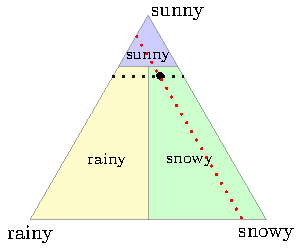
\includegraphics[width=0.3\textwidth]{tikz/t-example.pdf}
	\caption{A meteorology example with a bias towards citizen safety.}
	\label{fig:t-example}
\end{figure}

\subsection{Variance (Q4)}
\begin{corollary}
	\label{cor:variance}
	Let $\P$ be a set of continuous Lebesgue densities on $\Y=\reals$ with all $p \in \P$ having the same support.
	If there exist $p,q,q'\in\P$ with $\E_p Y = \E_q Y \neq \E_{q'} Y$ and $\Var(p) \neq \Var(q)$,
	\btw{Raf: I think this condition is tight actually: if there is no such triple in $\P$, I think $\eliccvx(\Var) \leq 1$ (i.e., $\Var$ is constant or a function of the mean)}
	then $\conscvx(\Var)=\eliccvx(\Var)=2$.
\end{corollary}
\begin{proof}
	For the upper bound, we may elicit the first two moments via the convex loss $L(r,y) = (r_1-y)^2 + (r_2-y^2)^2$, and recover the variance via $\psi(r) = r_2-r_1^2$, giving $\eliccvx(\Var) \leq 2$.
	Now for the lower bound.
	Without loss of generality, $\E_qY < \E_{q'}Y$.
	Let $r = \tfrac 1 2 \E_qY + \tfrac 1 2 \E_{q'}Y$, and define $V:\Y\to\reals, y\mapsto y-r$.
	Then $\zeros{V} = \{p'\in\P \mid \E_{p'}Y=r\} = \Gamma_r$ where $\Gamma:p'\mapsto \E_{p'}Y$ is the mean.
	As $\E_q Y < r < \E_{q'} Y$, we conclude $\E_q V < 0 < \E_{q'} V$.
	We have now satisfied Condition~\ref{cond:v-interior} for $d=1$.
	To apply Theorem~\ref{thm:bayes-risk-lower-bound}, it remains to show that $\Var$ is non-constant on $\Gamma_r$.
	% and the identity $\Var(p') = \E_{p'} Y^2 - (\E_{p'} Y)^2$
	By our assumptions and the definition of $\Var$, we have $\E_p Y^2 \neq \E_q Y^2$.
	Letting $p_1 = \tfrac 1 2 q + \tfrac 1 2 q'$, $p_2 = \tfrac 1 2 p + \tfrac 1 2 q'$, we have $\E_{p_i}Y = r$ for $i\in\{1,2\}$, but $\E_{p_1} Y^2 = \tfrac 1 2 \E_qY^2 + \tfrac 1 2 \E_{q'}Y^2 \neq \tfrac 1 2 \E_pY^2 + \tfrac 1 2 \E_{q'}Y^2 = \E_{p_2}Y^2$.
	As $p_1,p_2$ have the same mean but different second moments, we conclude $\Var(p_1) \neq \Var(p_2)$.
\end{proof}




\end{document}
%%% Local Variables:
%%% mode: latex
%%% TeX-master: t
%%% End:
